% %%%%%%%%%%%%%%%%%%%%%%%%%%%%%%%%%%%%%%%%%%%%%%%%%%%%%%%%
% Agentic Graph Reasoning --- two-column journal version of the M.Sc. Engg.
% (CSE) thesis in thesis_book/.
%
% SOURCE     : the thesis book is the source of truth. Every number here is
%              one the book states, and the book's numbers come from
%              results/phase4/thesis_numbers.json. Nothing is transcribed
%              from the run logs directly.
%
% REGISTER   : the book's. Short sentences with one idea each and plain
%              connectives. No colon explanations, no em-dashes, no
%              contractions, and at most two sentences joined into one.
%              British spelling, as in the book.
%
% BUDGET     : 20 to 22 pages including the references, and at most 1.5
%              pages of references.
%
% LAYOUT     : type sizes follow two model papers in
%              thesis_templates/references/. See preamble.tex.
%
% BUILD      : latexmk -pdf journal_0421052099.tex
% %%%%%%%%%%%%%%%%%%%%%%%%%%%%%%%%%%%%%%%%%%%%%%%%%%%%%%%%

\documentclass[10pt,twocolumn,a4paper]{article}

% !TEX root = journal_v2_0421052099.tex
%
% Packages and styles for the two-column journal version of the thesis.
%
% The class is the standard article class in two columns. Its type sizes copy
% two published papers the author chose as models. Both are kept in
% thesis_templates/references/.
%   - "A survey of graph meets large language" (IJCAI 2024) gives the title,
%     author, and affiliation styles, and most sizes. Body, abstract, and
%     reference text are 10 pt. Captions and footnotes are 9 pt. Section heads
%     are 12 pt bold and subsection heads 11 pt bold.
%   - "KBQA-o1" (ICML 2025) gives the 1 pt rules above and below the title,
%     with its spacing of 0.25 in, 0.22 in, and 0.3 in. Its tables are set at
%     8 pt or 9 pt, and so are these.
% Both papers are on US Letter. This one keeps A4, with the survey's 7 in text
% width and 0.25 in column gap.

\usepackage[a4paper, textwidth=7in, columnsep=0.25in, top=1in, bottom=1in,
  heightrounded]{geometry}

% Times text with Computer Modern maths, as in both model papers and the book.
% The book marks identifiers in sans and scales Helvetica to 92% so that it
% matches Times optically. The journal keeps the same pairing.
\renewcommand{\rmdefault}{ptm}
\usepackage[scaled=0.92]{helvet}
\renewcommand{\ttdefault}{pcr}

\usepackage{cite}
\usepackage{amsmath,amssymb}
\usepackage{array}
\usepackage{booktabs}
\usepackage{algorithm}
\usepackage{algorithmic}
\usepackage{tikz}
\usepackage{pgfplots}
\pgfplotsset{compat=1.18}
\usetikzlibrary{arrows.meta,positioning,calc,fit,backgrounds}
\usepackage{microtype}
\usepackage{etoolbox}
\usepackage{enumitem}
\usepackage[font=small, labelsep=colon, skip=4pt]{caption}
\captionsetup[table]{position=top}

\makeatletter

% Section heads as in the survey. 12 pt bold, then 11 pt bold, numbered
% "1 Introduction" and "1.1 Title". A head that runs to two lines is set
% ragged right, so its first line is not stretched.
\renewcommand\section{\@startsection{section}{1}{\z@}%
  {-12pt \@plus -3pt \@minus -2pt}{5pt \@plus 1pt}%
  {\normalfont\large\bfseries\raggedright}}
\renewcommand\subsection{\@startsection{subsection}{2}{\z@}%
  {-9pt \@plus -2pt \@minus -1pt}{4pt \@plus 1pt}%
  {\normalfont\fontsize{11}{13}\selectfont\bfseries\raggedright}}

% Footnotes are 9 pt, as in both model papers. The patch must come before
% hyperref, which wraps \@footnotetext.
\patchcmd{\@footnotetext}{\footnotesize}{\small}{}%
  {\PackageWarning{preamble}{Footnote size patch failed}}

% The title block. The title sits between two 1 pt rules, as in KBQA-o1. The
% author names are 12 pt bold and the affiliation 12 pt roman, as in the
% survey. The notes go at the foot of the first column without a number.
\newcommand\affiliation[1]{\gdef\agr@affiliation{#1}}
\newcommand\agr@titlenotes{}
\newcommand\titlenote[1]{\g@addto@macro\agr@titlenotes{\footnotetext{#1}}}
\renewcommand\maketitle{%
  \twocolumn[{%
    \centering
    \hrule height 1pt
    \vskip 0.25in
    {\Large\bfseries\@title\par}%
    % KBQA-o1 puts the rule 16 pt below the last title baseline. The depth of
    % that line already gives 2.6 pt of it.
    \vskip 13.2pt
    \hrule height 1pt
    \vskip 0.3in
    {\large\bfseries\@author\par}%
    \vskip 4pt
    {\large\agr@affiliation\par}%
    \vskip 0.35in
  }]%
  \thispagestyle{plain}%
  \begingroup
    \renewcommand\thefootnote{}%
    \agr@titlenotes
  \endgroup}

% The abstract sits in the first column under a centred 12 pt bold head, set
% in from both sides by 20 pt, as in both model papers.
\renewenvironment{abstract}{%
  \par\noindent\hfil{\large\bfseries\abstractname}\hfil\par
  \vskip 6pt
  \list{}{\leftmargin 20pt \rightmargin 20pt \listparindent 1em
    \itemindent \z@ \parsep \z@ \topsep \z@ \partopsep \z@}%
  \item\relax}%
  {\endlist}
\newcommand\keywords[1]{%
  \begin{list}{}{\leftmargin 20pt \rightmargin 20pt \itemindent \z@
    \parsep \z@ \topsep 6pt \partopsep \z@}%
  \item\relax\textbf{Keywords:} #1%
  \end{list}\vskip 6pt}

% Reference entries are separated by a small gap rather than the list default.
\apptocmd{\thebibliography}{\setlength{\itemsep}{1.5pt \@plus 0.5pt}%
  \setlength{\parsep}{\z@}}{}%
  {\PackageWarning{preamble}{Bibliography spacing patch failed}}

% IEEEtran.bst reads its options from a control entry that \bstctlcite cites.
% IEEEtran.cls defines the command. This is its definition, for other classes.
\def\bstctlcite{\@ifnextchar[{\@bstctlcite}{\@bstctlcite[@auxout]}}
\def\@bstctlcite[#1]#2{\@bsphack
  \@for\@citeb:=#2\do{%
    \edef\@citeb{\expandafter\@firstofone\@citeb}%
    \if@filesw\immediate\write\csname #1\endcsname{\string\citation{\@citeb}}\fi}%
  \@esphack}

\makeatother

% Floats may fill more of a page than the article defaults allow, as in
% IEEEtran. Without this, most of the wide tables would go to float pages.
\renewcommand{\topfraction}{0.9}
\renewcommand{\dbltopfraction}{0.9}
\renewcommand{\textfraction}{0.1}
\renewcommand{\floatpagefraction}{0.8}
\renewcommand{\dblfloatpagefraction}{0.8}
\setcounter{topnumber}{3}
\setcounter{dbltopnumber}{2}
\setcounter{totalnumber}{4}

% A column that breaks early before a float or a head is left a line short
% rather than stretched. Stretching opened blank lines between paragraphs.
\raggedbottom

% Lists are set close to the text, as in the model papers.
\setlist{topsep=3pt plus 1pt, itemsep=1pt, parsep=0pt, partopsep=0pt}
\setlist[itemize,enumerate]{leftmargin=1.5em}

\usepackage[hidelinks]{hyperref}
\usepackage[capitalise,nameinlink]{cleveref}

% URLs in the text face, as in the survey.
\urlstyle{same}

% Two columns are narrow. A little emergency stretch lets TeX set a line with
% a long identifier in it rather than push it into the margin.
\setlength{\emergencystretch}{1.5em}

% Names split only where their parts join, or not at all.
\hyphenation{WebQSP Complex-Web-Questions GraphRAG HippoRAG StructGPT}

% Fixed-width table columns set ragged right, as in the book.
\newcolumntype{L}[1]{>{\raggedright\arraybackslash}p{#1}}

% Figure palette and plot style, copied from thesis_book/buetcsepgthesis.sty
% so that the generated figures render here exactly as they do in the book.
% Okabe-Ito colours, and every series also differs by mark shape, so a
% greyscale print keeps them apart.
\definecolor{agrNode}{HTML}{0072B2}
\definecolor{agrSup}{HTML}{009E73}
\definecolor{agrUns}{HTML}{D55E00}
\pgfplotsset{
  agrplot/.style={
    width=0.46\textwidth,
    height=52mm,
    tick label style={font=\scriptsize},
    label style={font=\small},
    title style={font=\small\bfseries},
    legend style={font=\scriptsize, draw=none, fill=none},
    grid=major,
    grid style={gray!25, very thin},
    axis line style={gray!60},
    tick align=outside,
    tick style={gray!60},
  }}

% cleveref's names. Figures and tables are named in full, as in the survey.
\crefname{algorithm}{Algorithm}{Algorithms}
\Crefname{algorithm}{Algorithm}{Algorithms}
\crefname{equation}{Eq.}{Eqs.}
\Crefname{equation}{Eq.}{Eqs.}

\endinput


\hypersetup{
  pdftitle={Knowledge Graph Navigation and Structural Claim Verification for
    Multi-Hop Question Answering},
  pdfauthor={Md. Sakif Khan, Sadia Sharmin},
  pdfkeywords={Knowledge graphs, question answering, large language models,
    retrieval-augmented generation, hallucination, claim verification, agents}}

\title{Knowledge Graph Navigation and Structural Claim Verification\\
for Multi-Hop Question Answering}

\author{Md.~Sakif~Khan$^{\dagger}$, Sadia~Sharmin}

\affiliation{Department of Computer Science and Engineering\\
Bangladesh University of Engineering and Technology, Dhaka, Bangladesh}

\titlenote{$^{\dagger}$Corresponding author (sakifkhanopu@gmail.com).}
\titlenote{This paper is based on the first author's M.Sc.\ Engg.\ thesis.}

\begin{document}

\bstctlcite{IEEEexample:BSTcontrol}

\maketitle

\begin{abstract}
Large language models answer factual questions fluently. But they sound just
as fluent when they do not hold the facts. Retrieval-augmented generation
grounds answers in retrieved text, but retrieves once, before reasoning starts.
Systems that navigate a knowledge graph do better by interleaving retrieval
with reasoning. Even they send out whatever their final generation call
produces, and nothing checks the answer's claims before it reaches the user.
We propose Agentic Graph Reasoning (AGR), a knowledge-graph question-answering
framework whose agent plans sub-objectives and walks the graph through a
deterministic tool API. Before the answer is emitted, a Structural Verification
Layer splits the draft into atomic claims and checks each one against the
triples the agent traversed. We evaluate AGR on $400$ certified questions from
each of WebQSP and ComplexWebQuestions, against four baselines sharing one
frozen backbone and one call budget. AGR reaches a Hits@1 of $0.755$ on WebQSP
and $0.522$ on ComplexWebQuestions, beating every baseline at half the calls of
the agentic baseline. That baseline leads on the questions it finishes, so the
margin is affordability under a fixed budget. On ComplexWebQuestions, AGR is
the only system whose accuracy rises with hop count. An ablation finds one
detectable effect, opposite to what we expected. Removing the planner improves
WebQSP accuracy. The verification layer does not change how often AGR is right.
It makes answers auditable. A hand reading of all $256$ remaining failures
names the \emph{echo attractor}, a grounded entity next to the answer that
several systems fall into together.
\end{abstract}

\keywords{Knowledge graphs, question answering, large language models,
retrieval-augmented generation, hallucination, claim verification, agents.}

% !TEX root = ../journal_v2_0421052099.tex
%
% Condensed from thesis_book/chapters/introduction.tex.
\section{Introduction}\label{sec:intro}

\IEEEPARstart{L}{arge} language models answer factual questions fluently. But
often enough they give wrong answers, and those errors are not random. They are
systematic, and the model states them with the same confidence it gives a
correct answer~\cite{huang2025survey}. So a fabricated answer looks exactly like
a correct one. Things get worse when the answer requires putting several facts
together. A \emph{multi-hop} question such as ``Who directed the film that won
Best Picture in 1998?'' needs a chain of lookups in a fixed order. If the first
hop lands on the wrong entity, the rest of the chain carries on from a false
premise. And a check on the final answer alone never sees the intermediate
results.

Hallucinations arise at three points, and each calls for a different kind of
intervention~\cite{huang2025survey}. Defects in the training data can be fixed
only by curating the corpus and retraining. The model itself stores what it
knows diffusely across its weights, with no reliable signal that separates a
memorised fact from a plausible continuation. The third point is the prompt, and
it is the one this work takes on. When the context supplied with a question
already carries the facts needed to answer it, the model does not have to fall
back on parametric recall. Retrieval augmentation rests on that premise, and so
does this work. Our contribution is in how that context is assembled, and in
what gets checked before the answer goes out.

Retrieval-augmented generation (RAG)~\cite{lewis2020retrieval} attaches the
model to an external corpus and lets it answer from retrieved passages. For a
multi-hop question, the ranking signal measures the wrong thing. The passage
holding the intermediate entity may bear little resemblance to the question. And
flat retrieval cannot represent the relationships that a compositional question
has to traverse~\cite{li2023survey}. A knowledge graph makes those relationships
explicit, so composing two facts becomes a traversal.
GraphRAG~\cite{edge2024local} exploits this, but it still retrieves
\emph{statically}. It fetches a neighbourhood once, before reasoning starts. A
fixed radius is then either too small to contain the answer or so large that the
relevant edges are buried. The natural response is to interleave retrieval with
reasoning. Think-on-Graph~\cite{sun2024think} set that pattern with model-guided
beam search over the graph. Later systems added decomposition, backtracking, and
generated relation paths~\cite{chen2024plan,luo2024reasoning}.

Agentic navigation is the right shape for the problem, and this paper adopts it.
Three things it leaves unsolved motivate the work.

\textbf{Nothing checks what the final answer asserts.} Agentic systems ground
their answers in the subgraph they traverse, and the entities they assert do
exist in the graph. The problem is not fabrication but \emph{precision}. An
entity can sit in the retrieved subgraph, have been retrieved correctly, and
still be the wrong answer. Every system we survey emits whatever its final
generation call produces from the traversed context. Post-hoc self-checking
reduces factual error in free-form generation~\cite{dhuliawala2024chain}. What
none provides is a claim-level check against the retrieved triples, carried out
\emph{before} the answer is emitted, inside a graph-navigating agent.

\textbf{The contribution of individual mechanisms is unquantified.} Agentic
systems are assemblies of decomposition, scoring, backtracking, and
self-correction. The literature tends to report them as wholes. So when one
beats a static baseline, the mechanism that produced the gain is rarely
established.

\textbf{Accuracy is reported without cost.} Every exploration step costs at
least one model call. An accuracy table that leaves cost out makes agentic
methods look better across the board. The honest picture is a trade-off.

We present Agentic Graph Reasoning (AGR), a knowledge-graph question-answering
framework built as an explicit state machine over a constrained, deterministic
graph tool API. Its distinguishing component is a \emph{Structural Verification
Layer}. Before anything is emitted, the layer splits the draft answer into
atomic claims. It checks each one against the (head, relation, tail) triples the
agent actually traversed. Claims it cannot ground are re-explored or withdrawn.
So where it cannot ground a claim, AGR hedges rather than asserts. And the
answers it does give come paired with the triples that support them.

Stated formally, the input is a natural-language question $q$ and a knowledge
graph $G = (E, R, T)$ with entities $E$, relation types $R$, and triples $T
\subseteq E \times R \times E$. The system returns an answer set $A \subseteq E$
together with a supporting triple set $S \subseteq T$. The set $S$ contains only
triples the system traversed in reaching $A$, and it is checked before $A$ is
emitted. Three properties set this apart from standard question answering over
knowledge graphs. The output is a pair, and its supporting triples are part of
the contract. That is what makes the reasoning auditable rather than merely
asserted. The support must also be traversed, which rules out justifying, after
the fact, an answer the system reached some other way. And the justification is
checked before the answer is emitted. So unsupported content can be dropped or
hedged instead of merely flagged. Three research questions follow.

\begin{itemize}
\item \textbf{RQ1:} Does agentic navigation improve multi-hop factual accuracy,
  and does the advantage grow with the number of hops?
\item \textbf{RQ2:} What does pre-generation verification contribute beyond
  graph navigation?
\item \textbf{RQ3:} Which components contribute what, at what token cost?
\end{itemize}

We answer them with a controlled evaluation. All five systems share one frozen
backbone, one knowledge environment, and one call budget. So any difference
between them comes from architecture, not model capacity. The paper makes four
contributions.

\begin{enumerate}
\item AGR and its Structural Verification Layer (\Cref{sec:framework}). The word
  \emph{structural} names what the check establishes and, in the same word,
  bounds it. The check asks whether an edge joins a claim's endpoints, not
  whether it is the edge the claim names.
\item A controlled comparison of five systems on $400$ certified questions from
  each of WebQSP~\cite{yih2016value} and
  ComplexWebQuestions (CWQ)~\cite{talmor2018web}
  (\Cref{sec:setup,sec:results}). It
  splits the margin over the agentic baseline into search quality and
  affordability under a fixed budget.
\item A component-level ablation with paired significance tests
  (\Cref{sec:ablations}). It finds that
  decomposition is stratum dependent. Removing the planner improves accuracy on
  the shallower benchmark and trends toward harming it on the deeper one.
\item A hand reading of all $256$ remaining failures (\Cref{sec:errors}). It
  names the \emph{echo attractor}, a recurring failure in which several systems
  sharing a graph and a backbone converge on the same grounded but wrong answer.
  It also counts the benchmark's own label defects, which adjudication separates
  from those convergences.
\end{enumerate}

The headline results are these. AGR leads every accuracy column on both
datasets, and all eight paired tests against the baselines reject. Where the
shared call cap lets the agentic baseline finish, that baseline is slightly
ahead. So the margin is affordability, not better resolution. Structural
hallucination is eliminated by graph navigation itself, since the agentic
baseline also reaches zero. And removing the verification layer changes the
correctness of two questions out of $398$. Its contribution is auditability
rather than accuracy.

One limit applies to every absolute number. The knowledge environment is a union
of per-question subgraphs, each pre-extracted to contain its own question's
answer. That makes it friendlier than full
Freebase~\cite{bollacker2008freebase}, and the accuracies are not comparable
with evaluations over full Freebase. The comparisons between systems are sound,
because every system navigates the same environment (\Cref{sec:threats}).

The rest of the paper is organised as follows. \Cref{sec:related} reviews
related work, and \Cref{sec:environment} describes the knowledge environment.
\Cref{sec:framework} specifies AGR. \Cref{sec:setup} gives the experimental
setup and \Cref{sec:results} the results. \Cref{sec:errors} reads the failures.
\Cref{sec:discussion} discusses the findings and their limits, and
\Cref{sec:conclusion} concludes.

\endinput

% !TEX root = ../journal_v2_0421052099.tex
%
% Condensed from thesis_book/chapters/background.tex. Six works the book does
% not survey (GNN-RAG, SubgraphRAG, ToG-2, GCR, Self-RAG, CRAG) are cited for
% currency. Their entries sit in the book's own .bib file.
\section{Related Work}\label{sec:related}

\subsection{Static Retrieval over Text and Graphs}

Retrieval-augmented generation~\cite{lewis2020retrieval} gives a language model
material retrieved at the moment it answers. The answer can then rest on that
evidence rather than on \emph{parametric} knowledge, the facts absorbed into the
model's weights. Dense retrieval encodes queries and documents into a shared
vector space~\cite{karpukhin2020dense}, and sentence encoders produce embeddings
suited to direct cosine comparison~\cite{reimers2019sentence}. Graph-based
retrieval swaps flat passages for structured context.
GraphRAG~\cite{edge2024local} builds a graph over a corpus and answers from
summaries of its communities. HippoRAG~\cite{gutierrez2024hipporag} ranks nodes
by a random walk that restarts from the query's entities. Other systems learn
the retriever, scoring candidates with a graph neural
network~\cite{mavromatis2024gnnrag} or retrieving a bounded subgraph with a
light-weight scorer~\cite{li2025subgraphrag}. All of them retrieve once, before
reasoning, so the context cannot be conditioned on what reasoning finds. The
distinction that matters here is not graph versus vector but \emph{static versus
interleaved}.

\subsection{Agentic Exploration of Knowledge Graphs}

Think-on-Graph~\cite{sun2024think} established \emph{training-free} agentic
question answering over knowledge graphs, in which the model is prompted and
never fine-tuned. The model performs iterative beam search over the graph, with
beam width and depth both set to three, and prunes relations and entities
itself. Its successor adds document retrieval at each step~\cite{ma2024tog2}.
Plan-on-Graph~\cite{chen2024plan} decomposes the question into sub-objectives.
Its reflection step decides both whether to self-correct and which entity to
backtrack to, which makes it the one surveyed system with genuine backtracking.
That self-correction operates on the search, not on the draft answer.
Reasoning-on-Graphs (RoG)~\cite{luo2024reasoning} fine-tunes a model to generate
relation paths and instantiates them in the graph. Its answers are faithful by
construction, and graph-constrained reasoning~\cite{luo2025gcr} takes the same
route. But the plan is generated once, with no mechanism to revise it when it
fails to instantiate. KG-Agent~\cite{jiang2024kgagent} drives a toolbox with an
instruction-tuned model. StructGPT~\cite{jiang2023structgpt} reads structured
data through specialised interfaces. Generate-on-Graph
(GoG)~\cite{xu2024generate} admits model-generated triples when the graph is
incomplete, whereas AGR admits only graph triples.

KBQA-o1~\cite{luo2025kbqao1} is the system closest to genuine tree search. It
wraps a ReAct-style~\cite{yao2023react} agent in full Monte Carlo Tree
Search~\cite{kocsis2006bandit,browne2012survey}, with policy and reward models,
rollouts, and value backpropagation. AGR has none of these. Its search is guided
best-first search with a bounded beam and
backtracking~\cite{hart1968formal,pearl1984heuristics}, and each candidate is
scored once. KBQA-o1 also shows what an ablation can attribute. Removing its
tree search drops its F1 on GrailQA~\cite{gu2021beyond} from $78.5$ to
$48.5$~\cite{luo2025kbqao1}. That attribution was possible only because its
authors removed one component at a time.

\subsection{Verification and Factuality}

Chain-of-Verification~\cite{dhuliawala2024chain} has the model draft a response,
plan verification questions, answer them, and regenerate. Multi-agent
debate~\cite{du2024improving} gets a related effect by having several model
instances critique one another. Both check against the model's own knowledge,
and models cannot reliably correct their own reasoning without outside
feedback~\cite{huang2024selfcorrect}. A second group critiques the retrieval.
Self-RAG~\cite{asai2024selfrag} emits reflection tokens that judge whether a
passage supports the output. Corrective RAG~\cite{yan2024crag} grades the
retrieved documents and triggers a fallback search.
Reflexion~\cite{shinn2023reflexion} conditions an agent's next attempt on a
critique of its failed one, and a self-correcting graph RAG system applies such
a loop to clinical decision support~\cite{hu2025selfcorrecting}.
FActScore~\cite{min2023factscore} breaks generated text into atomic facts and
checks each against a reference source. It is a metric rather than a control
step, and the groundedness metric of \Cref{sec:metrics} borrows its
decompose-then-verify protocol.

\subsection{Positioning}

\Cref{tab:mechanisms} compares the closest systems on the mechanisms that matter
here. Decomposition is well established. Backtracking exists in Plan-on-Graph,
and RoG is faithful by construction. But no surveyed system decomposes its draft
answer into atomic claims and checks each one against the retrieved triples
before responding. That slot is the one AGR fills.

Published accuracies are not used to rank systems in this paper, and
\Cref{tab:reported} lists them for orientation only. Backbones differ across
papers, some papers evaluate on sampled subsets, and answer-matching conventions
vary. The same methods drop sharply when run on smaller open-weight backbones,
and RoG and KG-Agent are fine-tuned on these benchmarks. Think-on-Graph's own
paper reports two variants that differ by $1.8$ and $1.9$ points on CWQ with the
same two backbones~\cite{sun2024think}. That gap is the order of many claimed
improvements in this literature. So the agentic baseline here is reimplemented
and run under controlled conditions (\Cref{sec:baselines}). The one published
comparison is reported with its differences stated (\Cref{sec:rog}).

\begin{table}[!t]
\caption{Mechanisms of the closest prior systems. No surveyed system checks the
  claims of its final answer against retrieved triples before responding.}
\label{tab:mechanisms}
\centering
\scriptsize
\setlength{\tabcolsep}{2.5pt}
\begin{tabular}{@{}lL{22mm}L{10.5mm}L{12mm}L{17mm}@{}}
\toprule
System & Exploration & Decom\-poses & Back\-tracks & Verifies before answering \\
\midrule
Think-on-Graph & Model-pruned beam search & No & No & No \\
Plan-on-Graph & Adaptive planning with reflection & Yes & Yes & The search, not the answer \\
RoG & Fine-tuned relation-path plans & Partly & No & Faithful by construction \\
KG-Agent & Fine-tuned tool selection & Implicitly & No & No \\
GoG & Search with generated triples & Yes & No & No \\
StructGPT & Interfaces read in turn & No & No & No \\
KBQA-o1 & Tree search over an agent & Implicitly & By tree revisits & No \\
\midrule
AGR (ours) & Guided best-first beam search & Yes & Yes & Yes, claim by claim \\
\bottomrule
\end{tabular}
\end{table}

\begin{table}[!t]
\caption{Hits@1 as each paper publishes it. These figures are not comparable
  with one another or with this paper. Backbones and protocols differ, and two
  of the systems are fine-tuned.}
\label{tab:reported}
\centering
\footnotesize
\begin{tabular}{@{}llrr@{}}
\toprule
System & Backbone & WebQSP & CWQ \\
\midrule
Think-on-Graph~\cite{sun2024think} & GPT-3.5 & $76.2$ & $57.1$ \\
& GPT-4 & $82.6$ & $67.6$ \\
Plan-on-Graph~\cite{chen2024plan} & GPT-3.5 & $82.0$ & $63.2$ \\
& GPT-4 & $87.3$ & $75.0$ \\
RoG~\cite{luo2024reasoning} & Fine-tuned LLaMA2-7B & $85.7$ & $62.6$ \\
KG-Agent~\cite{jiang2024kgagent} & Fine-tuned 7B & $83.3$ & $72.2$ \\
GoG~\cite{xu2024generate} & GPT-3.5 & $78.7$ & $55.7$ \\
& GPT-4 & $84.4$ & $75.2$ \\
StructGPT~\cite{jiang2023structgpt} & GPT-3.5 & $72.6$ & --- \\
\bottomrule
\end{tabular}
\end{table}

\endinput

% !TEX root = ../journal_v2_0421052099.tex
%
% Condensed from thesis_book/chapters/environment.tex and the knowledge-graph
% preliminaries of thesis_book/chapters/background.tex.
\section{The Knowledge Environment}\label{sec:environment}

Everything the agent can know, it knows from the graph. So the environment sets
a ceiling on how accurate any system can be. A result reported without that
ceiling is hard to interpret.

\subsection{Freebase and Mediator Nodes}

A knowledge graph $G = (E, R, T)$ stores facts as triples $(h, r, t)$, each
asserting that relation $r$ holds from head entity $h$ to tail entity $t$.
Triples are atomic, so a claim can be checked by testing for specific edges.
They are also composable, and a chain of them expresses a multi-hop relationship
that no single triple states. Freebase~\cite{bollacker2008freebase}, frozen
since 2016, is the substrate of the standard benchmarks. One of its features
changes every depth measurement. A \emph{mediator node} is an unnamed node
standing for one fact with more than two participants, with one edge to each
participant. That Rainn Wilson played Dwight Schrute in \emph{The Office} is
stored as a mediator with edges to the actor, the character, and the show. So a
relationship a user would describe as one hop is two edges in the graph.
Distances in this paper are in \emph{raw} hops, which count graph edges. One
\emph{logical} hop through a mediator is two raw hops.

\subsection{Hallucination, Defined Operationally}\label{sec:halluc}

``Hallucination'' means different things in different papers. This paper adopts
a narrow, operational definition tied to the environment. An \emph{asserted}
entity is one the system names in its answer. It is \emph{ungrounded} if it does
not exist in the graph, or exists but lies more than four hops from every topic
entity of the question. A \emph{claim} is a single statement drawn from the
answer that relates two entities. It is \emph{unsupported} if the traversed
triples do not entail it. Two consequences follow. The definition is relative to
the environment, so an entity absent from the graph is ungrounded even if it is
true in the world. And groundedness is not correctness. An answer can be
grounded in every entity and still be the wrong answer to the question.

\subsection{Construction}

The environment is the union of every per-question subgraph that the
Reasoning-on-Graphs distribution~\cite{luo2024reasoning} publishes for WebQSP
and ComplexWebQuestions, across all splits. So the questions and the graph come
from one distribution and are mutually consistent. Taking the union is not a
minor detail. A per-question subgraph on its own is close to an oracle. It was
extracted to contain the answer, so an agent searching it meets almost no
distractors. Merging every question's neighbourhood into one graph brings the
distractors back. \Cref{tab:environment} records the result. Mediators are
retained rather than collapsed, since systems that skip them lose the facts they
encode~\cite{xu2024generate}. They make up $63.7\%$ of the nodes.

Two consequences must be disclosed. The subgraphs were pre-extracted to
guarantee that answers are reachable, which makes the environment friendlier
than raw Freebase. And the distribution keys entities by name rather than by
Freebase identifier. So distinct entities that share a surface form are merged
into one node. Both bound the absolute numbers, and \Cref{sec:threats} returns
to them.

The graph is stored in Neo4j~\cite{robinson2015graph}, with each relation as a
native relationship type, and is queried in Cypher~\cite{francis2018cypher}.
Entity names and the relation vocabulary are embedded with the 384-dimensional
sentence encoder all-MiniLM-L6-v2~\cite{reimers2019sentence}. Relation names are
verbalised before embedding, so \textsf{people.person.place\_of\_birth} is
encoded as the phrase it means. Embeddings have a narrow role. They link
question phrases to entities and pre-rank relation candidates. They never
establish that a fact is true, a role that belongs to the triples alone.

Entity resolution is a three-stage cascade of exact, lexical, and vector
matching, each stage tried only if the previous one fails. Over all $7{,}149$
topic-entity mentions in both test sets, $99.86\%$ resolve at the exact stage.
The ten that do not are bare machine identifiers that the benchmark carries in
place of a name. So a failure in this environment cannot be blamed on the
resolver missing the question's topic. The graph and the benchmarks share their
name strings, though, so this shows only that the resolver loses nothing the
environment contains.

\begin{table}[!t]
\caption{The knowledge environment and its validation gate. Reachability is the
  share of test questions with a gold answer within four raw hops of a topic
  entity. It is the Hits@1 ceiling over each full test split.}
\label{tab:environment}
\centering
\small
\begin{tabular}{@{}lr@{}}
\toprule
Property & Value \\
\midrule
Entities & $2{,}592{,}892$ \\
Triples & $8{,}309{,}194$ \\
Distinct relation types & $7{,}058$ \\
Mediator nodes & $1{,}652{,}618$ ($63.7\%$) \\
Mentions resolved by exact match & $7{,}139$ of $7{,}149$ ($99.86\%$) \\
\midrule
Reachable, WebQSP test split & $1{,}584$ of $1{,}628$ ($97.3\%$) \\
Reachable, CWQ test split & $3{,}519$ of $3{,}531$ ($99.7\%$) \\
\bottomrule
\end{tabular}
\end{table}

\subsection{The Validation Gate}\label{sec:gate}

No experiment ran until the environment was certified. For every test question
we computed whether a gold answer is reachable from a topic entity within four
raw hops, by breadth-first search over undirected edges. The agent's tools look
in both directions, so the gate does the same. Reachability is $97.3\%$ on
WebQSP and $99.7\%$ on CWQ (\Cref{tab:environment}). It is the accuracy ceiling,
since no navigating system can find an answer it cannot reach. Existence and
reachability agree question for question. When a question is unanswerable here,
it is because its gold entities are absent, not because they are too far away.
Reachability was also re-verified directly in Cypher, independently of the code
that computed it.

Certifying reachability says nothing about answers that are not entities. The
import gives every node a single label, with no typed literal. Only $77$ nodes
carry a full date as their name and $175$ a bare year, together under $0.01\%$
of the graph and untyped. And the tool layer exposes no sorting or comparison
operator. So ``the earliest'' or ``the smallest'' cannot be computed even when
every candidate is present. These gaps define a class of questions that are
\emph{unanswerable in this environment}, those whose answer is a date, a
measured quantity, or a superlative selection. Missing one is not a reasoning
failure, and \Cref{sec:errors} counts how often it happens.

\endinput

% !TEX root = ../journal_v2_0421052099.tex
%
% Condensed from thesis_book/chapters/framework.tex. Checked against the code
% in agr/ (nodes.py, scorer.py, planner.py, budget.py, kg_tools.py).
\section{The AGR Framework}\label{sec:framework}

\subsection{The Controlled-Agent Pattern}

There are two ways to build a graph-navigating agent. The first hands the model
a set of tools through native function calling and lets it drive the loop
itself, in the style of ReAct~\cite{yao2023react}. The second inverts control.
The \emph{program} orchestrates the loop, calls the graph tools
deterministically, and consults the model only at decision points, through
constrained prompts that must return JSON. AGR uses the second. Every graph
operation is then logged by construction, and budgets are enforced in code
rather than requested in prompts. A malformed model response can spoil one
decision, but it cannot corrupt the control flow. The agency in AGR lives in the
decision policy. That policy decides which sub-objectives to pursue, which edges
look promising, whether a path is a dead end, and whether the draft answer is
supported.

\subsection{The State Machine}

AGR is a state machine of six nodes over a shared typed state, built with
LangGraph (\Cref{fig:statemachine}). The topology has cycles. Exploration loops
until the evaluator is satisfied, and verification can send the agent back to
explore. The verifier sits between the decision to answer and the answer itself.
There is no path from the evaluator to the answerer that does not pass through
verification.

\begin{figure}[!t]
\centering
% !TEX root = ../journal_v2_0421052099.tex
%
% Hand-drawn. The AGR state machine of the book's Figure 4.1
% (thesis_book/chapters/framework.tex), redrawn narrower so that it fits one
% journal column. Topology, labels and colours are the book's. Blue marks the
% agent nodes and green the verifier.
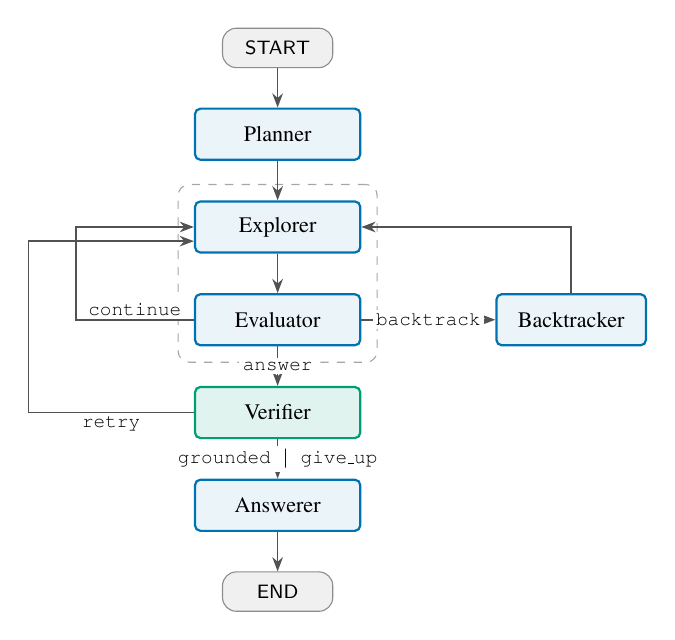
\begin{tikzpicture}[
    node distance=5mm,
    box/.style={draw=agrNode, thick, rounded corners=2pt, minimum height=6.5mm,
      fill=agrNode!8, minimum width=21mm, align=center, font=\footnotesize},
    vbox/.style={box, draw=agrSup, fill=agrSup!12},
    term/.style={draw=black!45, rounded corners=5pt, minimum height=5mm,
      minimum width=14mm, font=\scriptsize\sffamily, fill=black!6},
    flow/.style={-{Stealth[length=1.8mm]}, semithick, draw=black!68},
    lbl/.style={font=\scriptsize\ttfamily, inner sep=1.2pt, fill=white,
      anchor=center}]

  \node[term]              (start) {START};
  \node[box, below=of start] (plan) {Planner};
  \node[box, below=of plan]  (expl) {Explorer};
  \node[box, below=of expl]  (eval) {Evaluator};
  \node[vbox, below=of eval] (ver)  {Verifier};
  \node[box, below=of ver]   (ans)  {Answerer};
  \node[term, below=of ans]  (end)  {END};
  \node[box, right=17mm of eval, minimum width=19mm] (back) {Backtracker};

  \draw[flow] (start) -- (plan);
  \draw[flow] (plan) -- (expl);
  \draw[flow] (expl) -- (eval);
  \draw[flow] (eval) -- node[lbl] {answer} (ver);
  \draw[flow] (ver) -- node[lbl] {grounded $\mid$ give\_up} (ans);
  \draw[flow] (ans) -- (end);

  % The search cycle, from the evaluator back to the explorer.
  \draw[flow] (eval.west) -- ++(-15mm,0) node[lbl, above, pos=0.5]
    {continue} |- (expl.west);

  % The backtracking cycle, through the backtracker.
  \draw[flow] (eval.east) -- node[lbl] {backtrack} (back.west);
  \draw[flow] (back.north) |- (expl.east);

  % Verification-driven re-exploration.
  \draw[flow] (ver.west) -- ++(-21mm,0) node[lbl, below, pos=0.5] {retry} |-
    ([yshift=-1.8mm] expl.west);

  \begin{scope}[on background layer]
    \node[draw=black!35, dashed, rounded corners, inner sep=2mm,
          fit=(expl)(eval)] {};
  \end{scope}
\end{tikzpicture}

\caption{The AGR state machine. The dashed region is the explorer--evaluator
  search loop. The backtracker restores an earlier frontier, and the verifier's
  retry edge is verification-driven re-exploration. All three cycles are bounded
  by the budgets of \Cref{tab:budget}. Every path from the evaluator to the
  answerer passes through the verifier.}
\label{fig:statemachine}
\end{figure}

\subsection{The Graph Tool API}\label{sec:tools}

The model never writes graph queries. A generated query introduces a failure
that is indistinguishable, in the results, from a reasoning failure. When a
question is answered wrongly, one cannot tell whether the agent reasoned badly
or emitted invalid syntax. So the tools are parameterised Cypher templates,
written once and unit-tested. Four operations are live.

\textsf{search\_entity} links a mention to candidate nodes through the resolver
of \Cref{sec:environment}. It is the only entry point from text to graph.

\textsf{get\_relations} returns the relation types incident to an entity in
\emph{both} directions, each with its fanout count. Freebase's edge direction is
a modelling artefact. And the count is free signal, since a relation with a
fanout of forty thousand rarely answers a specific question. Relations in
administrative namespaces such as \textsf{common}, \textsf{type}, and
\textsf{freebase} are dropped. The list is capped at $300$ relations, sorted by
fanout.

\textsf{get\_neighbors} expands an entity along one relation. When it reaches a
mediator, it hops through it and returns the entities on the far side, each with
the chain of relations that reached it. So the model reasons about logical
neighbours, while the log keeps the raw chain. At most $200$ neighbours are
returned per expansion.

\textsf{verify\_connection} asks whether two entities are adjacent in the full
graph, directly or through one mediator. It ignores the relation and the
direction. A fifth operation, \textsf{verify\_triple}, also matched the
relation. It was built first as the claim checker and did not survive contact
with generated text. Claim decomposition produces relations phrased in English,
while Freebase predicates are neither phrased that way nor reliably one edge
long. So requiring the relation to match rejected claims that were true, and no
node calls it.

\subsection{Planner, Explorer, and Scorer}\label{sec:explorer}

The planner makes one model call. It turns the question into an ordered chain of
at most four sub-objectives, in which later objectives refer back to earlier
results with a \textsf{\#N} back-reference. The prompt is few-shot, with one
example for each of four archetypes (single hop, composition, conjunction, and
superlative). The single-hop example shows that \emph{not} decomposing is a
valid output. The plan is validated rather than trusted. If it is empty, too
long, refers forwards, or names no topic, the planner falls back to a single
sub-objective holding the whole question. Planning can degrade but can never
abort a run. Search is seeded from the dataset's annotated topic entities, the
standard protocol in this literature~\cite{sun2024think,luo2024reasoning}. That
choice separates reasoning from entity linking.

The explorer performs one expansion of the frontier. It pushes a checkpoint onto
the backtrack stack and gathers the relations of every anchor into a single
candidate list. It scores the whole list in one pass and takes the best three
edges per anchor, skipping banned ones. Each selected edge is expanded, and the
new frontier is sorted by the score of the edge that produced each entity and
truncated to five anchors. Each candidate edge $c$ receives the hybrid score
\begin{equation}\label{eq:score}
\mathrm{score}(c) = \alpha \cos\big(\mathbf{v}_{\mathrm{rel}(c)},
\mathbf{v}_{\mathrm{obj}}\big) + (1-\alpha)\,\mathrm{LLM}(c),
\end{equation}
where $\mathbf{v}_{\mathrm{rel}(c)}$ embeds the candidate's relation and
$\mathbf{v}_{\mathrm{obj}}$ embeds the active sub-objective. $\mathrm{LLM}(c)
\in [0,1]$ is the model's rating of how likely following the edge is to advance
that objective. Three properties matter. The objective is embedded, not the
question, with any back-reference already replaced by the resolved entity's
name. That substitution is the mechanism by which decomposition is supposed to
help. The model rates only the twenty candidates that the embedding ranks
highest, in one batched call. Every other candidate scores $\mathrm{LLM}(c) =
0$, so the pre-filter is a hard gate. And the blend is applied after the call.
The scoring prompt holds no configuration value, so every condition of an
$\alpha$ sweep shares the same cached model responses. We use $\alpha = 0.7$,
chosen on development data (\Cref{sec:ablation-setup}).

\subsection{Evaluator and Backtracking}

The evaluator makes one model call per expansion. It sees the active
sub-objective, the thirty traversed facts most relevant to it, and the remaining
budget. It decides whether to continue, backtrack, or answer, and it names the
entities that satisfy the objective. Those names are not taken on trust. Any
name that is not the tail of a traversed triple is discarded. A language model
asked which entities satisfy an objective will happily list ones it knows from
training but never retrieved. This \emph{groundedness filter} refuses to let
that recall pass as evidence. On one question of an early smoke run, the
evaluator listed nine correct countries that appeared in no retrieved triple,
because the beam had gone down an unrelated branch. The filter rejected all
nine, and the system abstained. That cost a point, but it kept every proposed
entity tied to the graph. Surviving resolutions are added to the candidate
answers on every evaluation, whether or not the objective was judged complete.
When an objective completes, the plan advances and the resolved entities become
the next frontier.

Backtracking fires on the first of three triggers, checked in this order. Either
the last expansion produced no new triples, or the frontier's signal fell below
a threshold $\tau = 0.20$, or the evaluator judged the direction a dead end. The
first two cost nothing, so a mechanically hopeless frontier is abandoned without
asking the model. The signal compared against $\tau$ is the largest of three
quantities. They are the best blended score among the expanded edges, the best
raw embedding similarity over every candidate, and the best model rating. So the
trigger fires only when all three are weak. The backtracker restores the
\emph{highest-scoring} snapshot on the stack rather than the most recent one. It
also bans the (anchor, relation, direction) combinations of the last pass.
Without that ban list, a deterministic scorer facing a restored frontier would
select the same edges again until the budget ran out. \Cref{alg:nav} states the
whole navigation loop.

\begin{algorithm}[!t]
\caption{AGR navigation, with the verification layer abstracted}
\label{alg:nav}
\small
\begin{algorithmic}[1]
\REQUIRE question $q$, budgets, blend $\alpha$, threshold $\tau$
\ENSURE answer $A$ with supporting triples $S$
\STATE $P \gets \textsc{Plan}(q)$; \textbf{if} invalid \textbf{then}
  $P \gets [\,q\,]$
\STATE $F \gets \textsc{SeedAnchors}(q)$; $T, C, \mathit{stack},
  \mathit{ban} \gets \emptyset$
\WHILE{budgets permit}
  \STATE push $(F, \mathit{depth}, \sigma)$ onto $\mathit{stack}$
  \STATE $R \gets \bigcup_{e \in F} \textsc{GetRelations}(e)$
  \STATE score $R$ by \Cref{eq:score} against the active objective
  \STATE $E \gets$ best $3$ edges per anchor, excluding $\mathit{ban}$
  \STATE $T \gets T \cup \textsc{GetNeighbors}(E)$
  \STATE $F \gets$ best $5$ new entities by edge score
  \STATE $\sigma \gets$ the largest of the three signals of this pass
  \STATE $(d, \mathit{done}, \rho) \gets \textsc{Evaluate}(\text{objective},
    \textsc{TopFacts}(T))$
  \STATE $\rho \gets \rho \cap \textsc{Tails}(T)$; $C \gets C \cup \rho$
    \COMMENT{groundedness filter}
  \IF{$\mathit{done}$}
    \STATE advance $P$; \textbf{if} no objective remains \textbf{then}
      $d \gets \textsf{answer}$ \textbf{else} $F \gets \rho$
  \ENDIF
  \IF{no new triples \OR $\sigma < \tau$ \OR $d = \textsf{backtrack}$}
    \STATE $\mathit{ban} \gets \mathit{ban} \cup E$; restore the
      highest-scoring snapshot
  \ELSIF{$d = \textsf{answer}$}
    \STATE \textbf{break}
  \ENDIF
\ENDWHILE
\STATE $(A, S) \gets \textsc{VerifyAndAnswer}(q, T, C)$
  \COMMENT{\Cref{alg:verify}}
\RETURN $(A, S)$
\end{algorithmic}
\end{algorithm}

The implementation departs from this specification in one way that has a
measurable consequence. It is recorded rather than repaired, since repairing it
would change the frozen results. The backtracker bans the \emph{most recent}
pass but restores the \emph{highest-scoring} snapshot, which is often older. So
whatever was expanded in between stays unbanned, and the explorer can select it
again. Over the main test runs, $53$ explorer passes expanded a set of (anchor,
relation) pairs that the same question had already expanded. That is exactly the
repetition the ban list exists to prevent.

\subsection{Budgets and Termination}

\Cref{tab:budget} lists the budgets. They are enforced in the routers between
nodes and in the model client, never in prompts. The depth budget counts
explorer expansions. One expansion can cross a mediator, so it does not bound
the search at four raw hops. Every cycle in \Cref{fig:statemachine} passes
through a router that checks a counter which only moves one way. So no sequence
of model outputs can produce a run that never ends. Every model call is also
cached, keyed on the model, its sampling settings, and the full prompt. A cache
hit replays the original token counts, so a cached rerun reproduces the original
run's budget record exactly. Each run writes two logs. The tool log records
every graph operation with its arguments, result size, and latency. The run
record holds the answer, the draft, the verification outcome, every backtrack
with its trigger, the full decision trace, and the budget snapshot. It also
names the backbone, the budget configuration hash, the run configuration, and
the source commit. So any record found anywhere states what produced it.

\begin{table}[!t]
\caption{Budget configuration. The last two rows are caps in the tool layer that
  bound what the agent can see.}
\label{tab:budget}
\centering
\footnotesize
\begin{tabular}{@{}lrl@{}}
\toprule
Budget & Value & What it bounds \\
\midrule
\textsf{max\_depth} & $4$ & explorer expansions \\
\textsf{beam\_width} & $3$ & edges expanded per anchor \\
\textsf{max\_anchors} & $5$ & frontier size \\
\textsf{max\_backtracks} & $3$ & backtracks per question \\
\textsf{max\_llm\_calls} & $25$ & model calls per question \\
\textsf{max\_verify\_iters} & $2$ & repair iterations \\
\textsf{max\_seconds} & $300$ & wall-clock time \\
\midrule
\textsf{max\_relations} & $300$ & relations offered to the scorer \\
\textsf{max\_fanout} & $200$ & neighbours per expansion \\
\bottomrule
\end{tabular}
\end{table}

\subsection{Design Validation on a Smoke Set}\label{sec:smoke}

Twenty questions from the training and validation splits, never from test, were
used once to check the assembled framework's mechanics. The set was built to
exercise specific machinery rather than to sample the benchmarks. The first
end-to-end run answered roughly three or four of them correctly, and the final
configuration answers thirteen or fourteen. That interval is where several of
the mechanisms above were shown to be necessary. The first run's failures
collapsed into five systematic causes, and \Cref{tab:rootcauses} gives the
mechanism each one motivated. Its before-state was read from a console log that
was never committed. So these figures are given as ranges, and none of them
enters any result.

\begin{table}[!t]
\caption{Root causes of failure in the first end-to-end run on the smoke set,
  and the mechanism each one motivated.}
\label{tab:rootcauses}
\centering
\footnotesize
\begin{tabular}{@{}L{43mm}L{39mm}@{}}
\toprule
Observed failure & Mechanism introduced \\
\midrule
Backtracking was a no-op, since a restored frontier reproduced the same scores and decisions & A ban list on abandoned (anchor, relation, direction) combinations \\
\addlinespace
The fact window showed the thirty most recent triples, so a large expansion pushed the answer out of view & A fact window ranked by relevance to the objective \\
\addlinespace
A relation cap of $80$, sorted by fanout, hid precise low-fanout relations behind hub relations & The cap raised to $300$, and administrative predicates blocked \\
\addlinespace
Entities resolved while an objective was incomplete were discarded & Candidates accumulated on every evaluation \\
\addlinespace
The frontier was truncated in insertion order, so the agent drifted from the anchor that mattered & The frontier sorted by edge score before truncation \\
\bottomrule
\end{tabular}
\end{table}

The two confabulations of the first run came from a retrieval defect, not a
generation defect. Two questions about national currencies produced a confident
``United States Dollar''. The relation cap had hidden the currency relation, the
beam surfaced triples about national income per capita in dollars, and the
answerer matched the pattern. No retrieved triple supported the answer, and
nothing that examined the answer caught it. After the cap was raised, both
questions resolved correctly at roughly a third of the token cost. But a
claim-level check against the traversed triples would have caught them
regardless of the retrieval defect. That is the argument for verifying before
emitting.

\subsection{The Structural Verification Layer}\label{sec:verification}

The navigation loop ends with a set of traversed triples and a list of candidate
entities. Nothing in it constrains what the final answer \emph{asserts}. A final
generation call is free to name an entity that appeared in neither, as the
currency answers of \Cref{sec:smoke} did.

The response is to check the draft before it is emitted. Chain-of-Verification
and FActScore decompose and check after generation, and both take further model
output as evidence~\cite{dhuliawala2024chain,min2023factscore}. The layer
borrows their decomposition step and rejects their placement and their evidence.
Placing the check inside the loop has three consequences. The checker sees the
same evidence the drafter saw. A rejected claim can trigger more exploration
while budget remains. And the judge of whether a fact holds is the environment,
not a second opinion from the model that wrote the draft.

\textbf{Claim decomposition.} One model call produces three things at once. They
are a prose draft, the entities the draft asserts as the answer, and a
decomposition of the draft into atomic claims $\langle h, r, t \rangle$ over
entity names. The call sees at most sixty traversed triples, ranked by relevance
to the question, and up to twenty-five candidates. The prompt requires names to
be copied exactly from the facts, and it requires a hedged draft to carry no
claims. It also requires the answer entities to be specific entities of the kind
the question asks for. That rule was added after drafts such as ``the senators
from New Jersey are the United States Senate members associated with New
Jersey''. Such an answer is grammatically complete and semantically empty. The
relation slot $r$ is free text, since the model has no reliable way to name a
Freebase predicate. Decomposition is sparse. On the development set the drafter
emitted $121$ claims over $80$ questions, with a median of one per question. Ten
questions produced no claims at all, so for those ten the layer certified
nothing.

\begin{figure*}[!t]
\centering
% !TEX root = ../journal_0421052099.tex
%
% Copied unchanged from thesis_book/figures/fig_claim_path.tex. Hand-drawn (not
% generated): the path one atomic claim takes through the verification layer.
% Mirrors Algorithm 1 line for line, including which of the three routes
% records citable evidence.
%
% Colour is semantic, not decorative: blue marks a step that does work, green
% the supported bucket, vermillion the unsupported one. The palette is the same
% colour-blind-safe set the generated figures use, and every distinction is
% still carried by shape and position, so a greyscale print loses nothing.
% Defined here because this figure is hand-drawn and has no generator.
\definecolor{agrNode}{HTML}{0072B2} \definecolor{agrSup}{HTML}{009E73}
\definecolor{agrUns}{HTML}{D55E00}
% This figure is set at two different sizes in two different text fonts (the
% thesis body font and the slide font), and the node widths are in millimetres
% either way. Hyphenation is switched off inside the picture so a node cannot
% break a word in one document and not the other; widths below are the ones that
% hold every label on the line count it was drawn for in both.
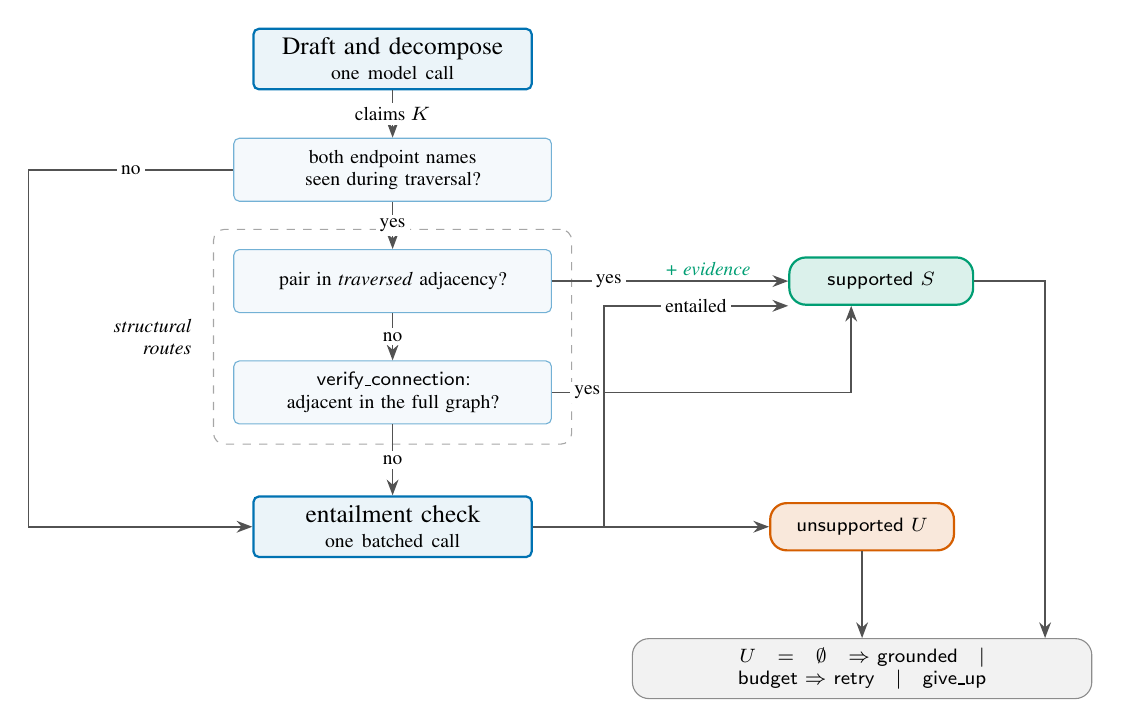
\begin{tikzpicture}[
    node distance=6mm,
    execute at begin picture={\hyphenpenalty=10000\exhyphenpenalty=10000},
    box/.style={draw=agrNode, thick, rounded corners=2pt, minimum height=7mm,
                text width=33mm, align=center, font=\small,
                fill=agrNode!8},
    dec/.style={draw=agrNode!55, rounded corners=2pt, minimum height=8mm,
                text width=38mm, align=center, font=\scriptsize,
                fill=agrNode!4},
    bucket/.style={draw, rounded corners=6pt, minimum height=6mm,
                text width=21mm, align=center, font=\scriptsize\sffamily},
    sup/.style={bucket, draw=agrSup, thick, fill=agrSup!14},
    uns/.style={bucket, draw=agrUns, thick, fill=agrUns!14},
    flow/.style={-{Stealth[length=2mm]}, semithick, draw=black!68},
    lbl/.style={font=\scriptsize, inner sep=1.5pt, fill=white},
    ev/.style={font=\scriptsize\itshape, inner sep=1.5pt, text=agrSup}]

  \node[box]                  (draft) {Draft and decompose
                                       \\[-2pt]{\scriptsize one model call}};
  \node[dec, below=of draft]  (d1)    {both endpoint names seen
                                       during traversal?};
  \node[dec, below=of d1]     (d2)    {pair in \emph{traversed}
                                       adjacency?};
  \node[dec, below=of d2]     (d3)    {\textsf{verify\_connection}:
                                       adjacent in the full graph?};
  \node[box, below=9mm of d3] (ent)   {entailment check
                                       \\[-2pt]{\scriptsize one batched call}};

  \node[sup, right=30mm of d2] (sup)  {supported $S$};
  \node[uns, right=30mm of ent] (uns) {unsupported $U$};

  \draw[flow] (draft) -- node[lbl, pos=0.5] {claims $K$} (d1);
  \draw[flow] (d1) -- node[lbl] {yes} (d2);
  \draw[flow] (d2) -- node[lbl] {no} (d3);

  % The one route that records evidence. "+ evidence" is the widest label on
  % the picture; at pos=0.80 its right edge crossed into the supported bucket,
  % so it is pulled back to the middle of the run instead.
  \draw[flow] (d2.east) -- node[lbl, pos=0.24] {yes}
              node[ev, pos=0.66, above] {+ evidence} (sup.west);
  % Arrives from BELOW, not along the bucket's own bottom edge. As "|- to
  % sup.south east" this turned at exactly the height the entailed route
  % turns at, ran on top of it as far as the bucket, then continued
  % underneath the bucket to land on its far corner: two arrows drawn over
  % each other and one of them apparently passing through a box.
  \draw[flow] (d3.east) -- node[lbl, pos=0.28] {yes} ++(16mm,0)
              -| ([xshift=8mm]sup.south west);
  \draw[flow] (d3) -- node[lbl] {no} (ent);
  % Endpoint never traversed: skip both structural routes entirely. The run is
  % long enough to clear the "structural routes" caption, which sits to the
  % left of the dashed region at the same height as this line's descent.
  \draw[flow] (d1.west) -- ++(-26mm,0) node[lbl, pos=0.5] {no} |- (ent.west);

  \draw[flow] (ent.east) -- ++(9mm,0) coordinate (e)
              |- node[lbl, pos=0.75] {entailed} (sup.south west);
  \draw[flow] (e) -- (uns.west);

  \node[bucket, draw=black!45, fill=black!5, below=11mm of uns.south,
        anchor=north, text width=56mm]
        (route) {$U = \emptyset \Rightarrow$ \textsf{grounded}\quad$\mid$\quad
                 budget $\Rightarrow$ \textsf{retry}\quad$\mid$\quad
                 \textsf{give\_up}};
  \draw[flow] (uns) -- (route);
  % Down into the routing box's top edge, near its right corner.
  % "-- ++(7mm,0) |- (route.east)" put the descent 7mm right of the bucket,
  % which is still well inside the routing box: the line came down through
  % the box's interior and the arrowhead sat on its border pointing
  % outwards, which is what it looked like -- an arrow leaving the box.
  % Turning down INSIDE route.east rather than outside it keeps the fix
  % from widening the picture; routed round the outside instead, the paper
  % -- which sets this figure unscaled -- went 25.8pt overfull.
  \draw[flow] (sup.east) -| ([xshift=-6mm]route.north east);

  \begin{scope}[on background layer]
    \node[draw=black!35, dashed, rounded corners, inner sep=2.5mm,
          fit=(d2)(d3), label={[font=\scriptsize\itshape, anchor=west,
          xshift=1mm]west:}] (strbox) {};
  \end{scope}
  \node[font=\scriptsize\itshape, left=1.5mm of strbox, align=right,
        text width=17mm] {structural\\routes};
\end{tikzpicture}

\caption{The path of one atomic claim through the verification layer, mirroring
  \Cref{alg:verify}. A claim leaves at the first test that settles it. Only the
  first structural route adds to the evidence, which is why some grounded
  answers carry supporting triples and others do not. A claim that names an
  entity the agent never traversed skips both structural routes, because the
  name map is built from traversed triples alone.}
\label{fig:claim}
\end{figure*}

\textbf{Two-stage checking.} \Cref{alg:verify} gives the procedure, and
\Cref{fig:claim} draws one claim's path through it. The structural check first
maps a claim's names back to nodes through the traversed triples alone. A claim
naming an entity the agent never traversed cannot reach either structural route.
It falls to the entailment check. The first structural route is \emph{traversed
adjacency}. The claim is supported if a traversed triple joins its endpoints,
and every such triple is attached to the answer as evidence. The second route
asks \textsf{verify\_connection} whether the endpoints are adjacent in the full
graph, since the agent may have reached both along different branches. It
records no evidence. This second route is rare. On the test sets it was
consulted for $100$ of the $2{,}110$ claims and accepted $39$. Claims that fail
both routes go to the \emph{entailment check}, one batched model call that
judges each claim against the same fact window. If that call fails for any
reason, every pending claim is marked unsupported.

The structural check runs first for three reasons. The graph should decide where
it can, so the model is consulted only where the graph is silent. Only traversed
adjacency yields triples that can be attached to the answer. And a set lookup is
free, while the entailment call is the layer's only unavoidable cost beyond
drafting.

\begin{algorithm}[!t]
\caption{Structural verification of a draft}
\label{alg:verify}
\small
\begin{algorithmic}[1]
\REQUIRE question $q$, traversed triples $T$, candidates $C$
\ENSURE draft, answer entities $A$, claim sets $S$ and $U$, evidence $E$
\STATE $W \gets \textsc{TopFacts}(q, T, 60)$
\STATE $\mu \gets$ name-to-id map over $T$
\STATE $(\mathit{draft}, A, K) \gets \textsc{DraftAndDecompose}(q, W, C)$
\STATE $\mathit{adj} \gets \{(h,t),(t,h) : (h,r,t) \in T\}$
\STATE $S \gets \emptyset$; $P \gets \emptyset$; $E \gets \langle\,\rangle$
\FORALL{$c = \langle h, r, t \rangle \in K$}
  \IF{$h \notin \mu$ \OR $t \notin \mu$}
    \STATE $P \gets P \cup \{c\}$ \COMMENT{never traversed}
  \ELSIF{$(\mu[h], \mu[t]) \in \mathit{adj}$}
    \STATE $S \gets S \cup \{c\}$; append the joining triples to $E$
  \ELSIF{$\textsf{verify\_connection}(\mu[h], \mu[t])$}
    \STATE $S \gets S \cup \{c\}$ \COMMENT{no evidence recorded}
  \ELSE
    \STATE $P \gets P \cup \{c\}$
  \ENDIF
\ENDFOR
\STATE $U \gets \emptyset$
\IF{$P \neq \emptyset$}
  \STATE split $P$ into $S$ and $U$ by $\textsc{Entail}(W, P)$
\ENDIF
\IF{$U \neq \emptyset$ \AND repair budget remains}
  \STATE add a repair objective for the first claim in $U$
\ENDIF
\STATE route \textsf{grounded} if $U = \emptyset$, else \textsf{retry}
  if the repair, depth, and time budgets remain, else \textsf{give\_up}
\RETURN $(\mathit{draft}, A, S, U, E)$
\end{algorithmic}
\end{algorithm}

\textbf{Repair.} The router after the verifier has three outcomes. With no
unsupported claim it routes to \textsf{grounded}, and the draft is emitted with
no further model call. With unsupported claims and the repair, depth, and time
budgets all remaining, it routes to \textsf{retry}. The verifier has already
appended a repair objective for the first unsupported claim and re-anchored the
search on that claim's head entity. Anything else routes to \textsf{give\_up}.
On that path the final entity list is computed deterministically. An entity is
kept if it appears in a supported claim or in no unsupported claim. One rewrite
call then restates the prose around the kept list. Repair is capped at two
iterations. The grounded path costs nothing, so the layer is cheap overall. On
the development set it raised mean tokens per question from $4{,}858$ to
$4{,}925$, about $1.4\%$.

The retry route never ran on the development set. On all three development
questions that produced an unsupported claim, the depth budget was already spent
when the verifier was reached. That correlation does not survive the move to
test. Across the $800$ test questions the verifier asked for a repair on $52$,
and exploration actually resumed on $28$ of them. So the depth condition blocks
the retry about half the time. Thirteen questions ended grounded after a repair,
and the iteration cap bound on $15$.

That deterministic filter replaced a second generation call, and the reason is
the most instructive result of the design. On the development set, a
question-by-question comparison against the same system with claim checking
switched off found exactly three questions that differed. No entailment verdict
was involved in any of them. All three traced to the rewrite call, which at the
time regenerated the answer entities along with the prose. In one case it
dropped four correct entities together with an unsupported one. In another it
added the question's own subject to the answer. In the third it respelled the
graph's \textsf{University Yale} as \textsf{Yale University}, which scored as
wrong (\Cref{sec:example}). The verification logic was sound, and its repair
path frequently was not. Replacing generation with filtering removed two of the
three regressions.

\textbf{The output contract and its limits.} AGR returns each answer paired with
the triples that support it. That coverage is narrower than the phrase suggests.
Only the traversed-adjacency route records evidence. And the run log keeps the
number of supporting triples, not the triples. So the contract holds inside the
run, but it cannot be checked afterwards from the committed records. On the
development set, $13$ of $80$ answers carry no supporting triples at all. Ten of
them are hedges with no claims, for which zero is the honest count. The other
three had every claim rejected or certified only through the route that records
nothing.

\subsection{A Worked Example}\label{sec:example}

The question ``Which university, founded in 1701, did actor James Franco
attend?'' shows the layer end to end. Its gold answer is the graph's
\textsf{University Yale}. Navigation anchors on James Franco and expands his
education relations. The plan's first objective, the university founded in 1701,
is never satisfied, because the environment holds essentially no date literals.
After three evaluator-triggered backtracks, the run stops on the depth budget.

The drafter writes ``James Franco attended University Yale, which was founded in
1701.'' Its entity list is \textsf{[University Yale]}, copied from the fact
window in the graph's spelling. It decomposes the draft into an attendance claim
and a founding claim. Traversed triples join the attendance claim's endpoints,
so that claim is supported, and four triples are recorded as its evidence. The
founding claim names \textsf{1701}, which no traversed triple mentions. So it
falls to the entailment check, which correctly reports it unsupported. The depth
budget is spent, so the router takes \textsf{give\_up}. The filter keeps
\textsf{University Yale}, since it appears in a supported claim. The rewrite
asserts the attendance and hedges the founding date, and the answer scores as a
hit.

The instructive part is the counterfactual. Before deterministic filtering, the
identical trace ended with \textsf{[Yale University]}. The rewrite call had
restated the answer in the model's own spelling rather than the graph's, and the
answer was scored wrong. The claim-level checks had worked perfectly. The layer
still emitted an entity string that appears nowhere in the environment, which is
the precise thing it exists to prevent.

\subsection{What the Layer Can Get Wrong}\label{sec:failure-modes}

The ways the layer can be wrong follow from its design, independently of how
often they occur. A claim is \emph{wrongly rejected} when the layer withholds
support that the environment would in fact provide. It is \emph{wrongly
accepted} when the layer certifies a claim that the environment does not
support. \Cref{sec:errors} reports which of these mechanisms actually fired.

Five mechanisms lead to wrongful rejection. The most expensive is the composite
claim. When a draft asserts a filtered set, such as ``these teams were founded
before 1996'', its claims are about the founding. The membership that makes each
team a candidate may never be claimed at all. So each team's only claim is the
unverifiable one, the filter drops every team, and a draft with four correct
answers becomes a hedge. A claim can also name an endpoint outside the
traversal, which skips both structural routes whatever the graph contains. The
entailment check's fact window is ranked for relevance to the question rather
than to the claim, so a peripheral claim may be judged against facts that never
mention it. A failed entailment call records an infrastructure error as a
rejection. And the name map keeps the first identifier it sees for a name, so
two entities that share a surface form collapse into one.

Wrongful acceptance has more mechanisms, and they reach further. Both structural
routes ignore the relation and the direction. So any edge between two entities
certifies any claimed relation between them. A claim that X is Y's mother is
accepted on an edge recording that X is Y's child. That is the price of
free-text relations, and it is the layer's main acceptance risk. On the test
sets the verifier accepted $2{,}008$ of the $2{,}110$ claims it decomposed. The
number accepted by a relation-blind test lies somewhere in $[39, 2{,}008]$. The
lower end is what the log pins down, and the upper end is what the mechanism
permits. The mediator hop adds a second looseness. An actor, a film, a
character, and a period are all mutually connected through one performance node,
so any claim relating two of them is certified. A draft with no claims has no
unsupported claim and is routed \textsf{grounded}, which describes $10$ of the
$80$ development questions. An entity that the drafter named but the decomposer
never put into a claim is never checked. So the guarantee over emitted entities
rests on decomposition recall, which is itself an unchecked model output. A
claim accepted structurally is never examined for meaning, since the entailment
check sees only what the structural routes could not resolve. And an answer
whose every claim is supported can still fail to answer the question, as the New
Jersey senators draft does. No claim-level check can catch that, because the
defect lies between the claims and the question.

The layer establishes that the entity pairs a draft relates are connected in the
environment. On the repair path it also makes the emitted entity list a
deterministic function of those verdicts rather than a second generation. It
does not establish that the claimed relation is the one the edge records, that
an entity absent from every claim was grounded, or that the answer is responsive
to the question. Those boundaries are properties of the design rather than
defects discovered in it.

\endinput

% !TEX root = ../journal_0421052099.tex
%
% Condensed from the setup half of thesis_book/chapters/evaluation.tex.
\section{Experimental Setup}\label{sec:setup}

Each research question is answered by a distinct experiment rather than by one
table read three ways. RQ1 is answered by the main comparison of five systems on
two datasets, scored with Hits@1 and F1, broken down by hop stratum, and tested
in pairs. The claim about multi-hop accuracy rests on the per-stratum breakdown,
not on the aggregate. RQ2 is answered by three measurements that disagree with
one another, and that disagreement is itself the finding. They are the two-tier
groundedness metric, the precision columns of the main comparison, and the
verifier ablation. RQ3 is answered by four ablations that each remove one
component, compared with the unmodified system on the same questions.

\subsection{Pre-Specification}

One rule governed everything from the moment the test files were built. Nothing
was tuned. No prompt was edited, no configuration value was changed, and no
threshold was adjusted after test data was touched. Four decisions were fixed in
writing before the measurements they govern. They were the frozen configuration
($\alpha = 0.7$, $\tau = 0.20$, claim verification on), the sample size of $400$
questions per dataset, a certification threshold for the retrieval baselines,
and a judge-agreement threshold of Cohen's $\kappa \geq 0.7$. The last was
missed by $0.0005$ and is reported as missed. Nothing was filed with a public
registry, so the claim is pre-specification rather than pre-registration.

\subsection{Datasets and Certified Test Samples}\label{sec:testsets}

WebQSP~\cite{yih2016value} holds natural questions from search logs, mostly one
or two hops from the topic entity, and multi-valued answers are common.
ComplexWebQuestions (CWQ)~\cite{talmor2018web} composes WebQSP questions into
deeper chains through SPARQL templates, with conjunctions, superlatives, and
comparisons. Running five systems over the full test splits of $1{,}628$ and
$3{,}531$ questions was projected to exceed the budget. So the evaluation fell
back to the pre-specified alternative, a sample of $400$ questions per dataset,
stratified by hop count at seed $42$. In the end the whole benchmark, ablations
included, cost \$11.13 in API spend.

The stratification variable is the length of the shortest path from any topic
entity to any gold answer, capped at four raw hops (\Cref{tab:testsets}). WebQSP
is $64\%$ one-hop, and its stratum of three or more hops holds four questions,
too few to interpret. CWQ is mostly two-hop, with a real deep tail of $49$
questions. The \textsf{unreachable} stratum is kept. Dropping it would raise
every score by the same amount and misdescribe the environment. The ceiling is
the share of questions with a reachable gold answer, and no system can score
above it on Hits@1. The two benchmarks also differ in their gold answer sets.
WebQSP averages $7.15$ gold entities per question, with a median of $1.5$ and a
largest question listing $237$. CWQ averages $1.75$ with a median of $1$.

\begin{table}[!t]
\caption{The two certified test samples by hop stratum. The ceiling is the share
  of the $400$ questions with a gold answer reachable within four raw hops.}
\label{tab:testsets}
\centering
\small
\setlength{\tabcolsep}{4.5pt}
\begin{tabular}{@{}lrrrrrr@{}}
\toprule
Dataset & $n$ & 1 hop & 2 hops & 3+ hops & Unreach. & Ceiling \\
\midrule
WebQSP & $400$ & $256$ & $128$ & $4$ & $12$ & $97.0\%$ \\
CWQ & $400$ & $137$ & $211$ & $49$ & $3$ & $99.2\%$ \\
\bottomrule
\end{tabular}
\end{table}

\subsection{Gold-Label Quality Control}\label{sec:gold}

Both benchmarks carry label defects, CWQ more, since its questions and answers
are generated by templates. A question whose gold answer is wrong is not a
system failure. Counting it as one corrupts both the accuracy tables and the
error analysis. The detection principle is consensus against gold. When at least
three of the five systems assert the same non-gold answer, the label is worth
examining. The voters are the five systems of the main comparison, spanning two
knowledge sources and four retrieval paradigms. The ablation conditions would
not do, since their agreement would describe one architecture rather than a
label. That pass flagged $58$ WebQSP and $47$ CWQ questions (\Cref{tab:gold}).
Adjudication confirmed $22$ and $19$ of them ($5.5\%$ and $4.8\%$ of the
samples) as a wrong gold label or an underdetermined question. The gap between
the flagged and the confirmed counts is not noise, and \Cref{sec:echo} explains
it.

\begin{table}[!t]
\caption{Gold-label adjudication. The pass emits one row per consensus answer,
  so rows and questions are different units. Exclusions are the questions judged
  to have a wrong gold label or an ambiguous question.}
\label{tab:gold}
\centering
\small
\setlength{\tabcolsep}{4pt}
\begin{tabular}{@{}lrrrrr@{}}
\toprule
Dataset & Rows & Flagged & Gold wrong & Ambiguous & Excluded \\
\midrule
WebQSP & $89$ & $58$ & $12$ & $10$ & $22$ ($5.5\%$) \\
CWQ & $59$ & $47$ & $17$ & $2$ & $19$ ($4.8\%$) \\
\bottomrule
\end{tabular}
\end{table}

Label errors come in two kinds with opposite evidence signatures, and telling
them apart is what makes the adjudication reproducible. A \emph{world-fact
error}, where the gold answer contradicts reality, shows \emph{mixed} consensus.
The parametric control and the graph-based systems agree against the label, so
two different knowledge sources agree. In one specimen, four systems answer
Bexar County for the seat of the San Antonio City Council, against a gold answer
of Comal County. An \emph{annotation-pipeline error}, where the gold answer
contradicts the very graph the labels came from, shows \emph{graph-only}
consensus. Asked who had a concert named Crazy Love Tour, the graph-reading
systems all return Michael Bubl\'{e}. The gold answer lists his professions,
because the annotation query traversed one relation too far.

The confirmed defects are removed from the failure census. The accuracy tables
are not rescored. Rescoring on self-adjudicated labels would replace one
contestable ground truth with another, and the defects cut both ways.
Recomputing every cell without them moves each system by between $+0.001$ and
$+0.020$ Hits@1 and changes no ranking.

\subsection{Backbone}\label{sec:backbone}

Every system runs on the same frozen backbone, \textsf{gpt-5.4-mini-2026-03-17},
at temperature $0$, with reasoning effort set to \textsf{none} and the response
cache enabled. A non-reasoning model keeps hidden reasoning tokens out of the
cost metric. Temperature zero on a hosted API is greedy rather than
deterministic, and a sequential agent amplifies a single divergent token. In a
qualification probe, the frozen model repeated its full decision sequence on $8$
of $12$ probes. The probe compared it with \textsf{gpt-4.1-mini-2025-04-14}, and
both models carried a persistent ungrounded answer. One asserted the United
States dollar for a question about the Dominican peso in two of four runs, and
the other named the wrong Beckham child in all four. Each also carried
intermittent ones, where the same question on the same graph moved between a
grounded correct answer and an ungrounded wrong one. Choosing a backbone does
not remove this class of error. It only moves it around, which is the premise of
this work. So reproducibility rests on the cache. Every table comes from one
recorded run per condition, which replays exactly from the cache. Run-to-run
variance is not measured, and \Cref{sec:threats} carries it as a limitation.

\subsection{Baselines}\label{sec:baselines}

Four baselines span the space between no retrieval and agentic navigation.

The \textbf{no-retrieval} control makes a single call with no facts and may
return an empty answer. WebQSP and CWQ predate current models and may sit in
their training data. So this control measures the floor that every retrieval
result is read against.

\textbf{Vector-RAG} verbalises every triple as a sentence, embeds it with
MiniLM~\cite{reimers2019sentence}, and answers from the top $30$ sentences in
one call. That is dense retrieval~\cite{karpukhin2020dense} applied to a graph.
A fact stored through a mediator has no single triple that expresses it, so no
retrieved sentence can express it either.

\textbf{Static GraphRAG} is the comparison with structure but without
navigation~\cite{edge2024local}. It expands a one-logical-hop neighbourhood
around the topic entities, reranks it by similarity to the question, and answers
from the top $30$ facts. It shares Vector-RAG's prompt, so the difference
between the two isolates the retrieval strategy. Its expansion keeps at most
$100$ edges per topic entity in no stated order, and at least one topic entity
is truncated on $72.5\%$ of questions.

\textbf{Think-on-Graph} is the agentic baseline~\cite{sun2024think},
reimplemented on this environment's tools. It uses beam width $3$, depth $3$,
model-based pruning of relations and entities, and a sufficiency check at each
depth. Holding the graph, model, and budget constant makes it a stronger
comparison than citing published numbers. It also makes its numbers incomparable
with the published ones. Two asymmetries are stated in advance. The baseline
stops its search one call before the shared limit and reserves that call for its
answer, where AGR makes no such reservation. And it keeps the first $40$
relations per entity and $20$ neighbours per relation, its own algorithm's
pruning widths, against AGR's $300$ and $200$. That cut binds on $31.6\%$ of the
entities it expands, against $1$ of AGR's $3{,}097$.

Every system shares the backbone, the environment and its relation blocklist,
the entity resolver, the question files, the $25$-call budget, and the output
schema. Two things are not shared. The baselines get a plain answering prompt,
while AGR's drafting prompt carries the provisions of \Cref{sec:verification}.
And the candidate widths differ, as just stated. Each retrieval baseline was
certified on development data before any test question ran. The pre-specified
failure was hedging while the gold answer sat in the baseline's own retrieved
facts, allowed on fewer than $15\%$ of hedges. Vector-RAG measured $0\%$ on both
datasets, and Static GraphRAG $10\%$ and $14\%$.

\subsection{Metrics}\label{sec:metrics}

Both accuracy metrics are computed over entity sets after Unicode NFKC
normalisation, case folding, and whitespace stripping, with no fuzzy matching.
\emph{Hits@1} is $1$ if any predicted entity matches any gold entity, which is
the convention in this literature. \emph{F1} is computed per question between
the predicted set $A$ and the gold set $A^{*}$ and averaged over questions, with
$P = |A \cap A^{*}| / |A|$, $R = |A \cap A^{*}| / |A^{*}|$, and $F_1 =
2PR/(P+R)$. Hits@1 rewards a system that names one correct entity among several
wrong ones. Precision charges for the rest. Strict matching does not manufacture
failures. Only $1$ of AGR's $65$ wrong answers on WebQSP and $6$ of its $99$ on
CWQ are surface-form near misses.

A \emph{hedge} is an empty answer set. It scores zero on both metrics, and the
hedge rate gets its own column, so the trade between abstention and accuracy
stays visible. \emph{Assertion precision} is the share of the questions a system
commits on that it answers correctly.

Groundedness is measured in two tiers, and the word \emph{tier} refers to this
metric and nothing else. \textbf{Tier~1} is structural and deterministic. An
asserted entity is grounded if and only if it exists as a node and lies within
four hops of a topic entity. It applies to every asserted entity in all
$4{,}000$ records. \textbf{Tier~2} asks whether the entity is supported \emph{as
the answer}. For $60$ asserted answers per system per dataset, a model judges
whether any of the three shortest graph paths between topic and answer expresses
the relationship the question asks about. Mere connectedness is not support. The
judge sees no system identity, gold answer, or score. The first author labelled
$100$ judged items blind, without opening the judge's verdicts or the answer key
until the labels were saved. Observed agreement was $85\%$, with near-symmetric
marginals ($54$ items supported by the human against $51$ by the judge) and
near-symmetric disagreement ($9$ against $6$). So neither rater is
systematically the more lenient. Cohen's $\kappa$~\cite{cohen1960coefficient}
corrects that agreement for chance,
\begin{equation}
\kappa = \frac{p_o - p_e}{1 - p_e} = \frac{0.8500 - 0.5008}{1 - 0.5008} = 0.6995,
\end{equation}
where $p_o$ is the observed agreement and $p_e$ the agreement expected by
chance. That is substantial agreement
on the conventional scale~\cite{landis1977measurement}. But it falls short of
the
pre-specified $0.7$ by $0.0005$, and it is reported as short. Re-judging a fresh
sample until the bar was cleared was available and was not taken, since
re-running until a threshold is met is exactly what pre-specification exists to
prevent. So no conclusion rests on Tier~2 alone. The judge also runs
on the same backbone as the systems it judges.

Tokens and calls are counted by the shared budget meter and are exact. Latency
is computed over cold-cache records only. Confidence intervals are $95\%$
percentile bootstrap intervals~\cite{efron1979bootstrap} from $10{,}000$
resamples. They are read as a sense of scale for a difference, not as a
hypothesis test, and they make no distributional assumption about per-question
F1. Paired comparisons use the exact form of McNemar's
test~\cite{mcnemar1947note} on per-question correctness. The test looks only at
the discordant pairs, the questions that one system answers correctly and the
other does not. Pairing matters here, because every system runs on the same
questions, and an unpaired test would throw that pairing away.

\subsection{Ablations and Development Tuning}\label{sec:ablation-setup}

Four conditions each remove one mechanism. \textbf{No-planner} installs the
whole question as the only sub-objective. \textbf{No-backtrack} sets the
backtrack budget to zero. \textbf{No-verifier} emits the draft without checking
any claim, with the drafting call unchanged. \textbf{Embedding-only} sets
$\alpha = 1$, which removes the model term from the scorer. The ablations run on
stratified halves of $200$ WebQSP and $198$ CWQ questions. The reference row is
the unmodified system restricted to the same questions. Accuracy on $400$
questions and on $198$ are different numbers for the same system, so comparing
against the full score would be invalid. The planner flag was the only code
change. It was certified as a no-op on the frozen path, since re-running an
answered question served every model call from the cache.

The two free parameters were tuned on $80$ development questions, disjoint from
both test samples. A joint sweep over $\alpha \in \{0.3, 0.5, 0.7, 1.0\}$ and
$\tau \in \{0, 0.20\}$ peaked at $\alpha = 0.7$, with $64$ of $80$ questions
correct against $61$, $62$, and $59$ at the other three weights
(\Cref{tab:sweep}). The curve is not clean. The wrong-answer column peaks at
$\alpha = 0.5$, where the system commits more often. The threshold $\tau$ barely
mattered at the values swept, and it was frozen at $0.20$ anyway. That is stated
plainly rather than dressed up as a tuned choice. Two further conditions
switched claim checking off. At the frozen weights the draft-only condition
scored $66$ hits to $64$. After the answer-entity filter of
\Cref{sec:verification} was corrected, still on development data, the frozen
condition scored $65$ hits, $11$ hedges, and $4$ wrong answers. So on this set
the layer cost one correct answer and removed no wrong one. The draft-only
condition was never re-run after the correction, so this is the closest
available reading rather than a matched pair. \Cref{sec:ablations} finds the
same thing at test scale.

\begin{table}[!t]
\caption{The development sweep, $n = 80$. Hits, hedges, and wrong answers
  partition the set. The last two rows switch claim checking off. All rows
  predate the correction to the answer-entity filter.}
\label{tab:sweep}
\centering
\small
\setlength{\tabcolsep}{3.5pt}
\begin{tabular}{@{}rrcrrrrrr@{}}
\toprule
$\alpha$ & $\tau$ & Verify & Hits & Hedge & Wrong & F1 & Tokens & Calls \\
\midrule
$0.3$ & $0.00$ & yes & $61$ & $12$ & $7$ & $0.728$ & $4{,}999$ & $7.4$ \\
$0.3$ & $0.20$ & yes & $61$ & $12$ & $7$ & $0.728$ & $5{,}030$ & $7.5$ \\
$0.5$ & $0.00$ & yes & $62$ & $10$ & $8$ & $0.743$ & $4{,}874$ & $7.2$ \\
$0.5$ & $0.20$ & yes & $62$ & $10$ & $8$ & $0.743$ & $4{,}874$ & $7.2$ \\
$0.7$ & $0.00$ & yes & $64$ & $11$ & $5$ & $0.769$ & $4{,}925$ & $7.3$ \\
$\mathbf{0.7}$ & $\mathbf{0.20}$ & \textbf{yes} & $\mathbf{64}$ & $11$ & $5$ & $0.769$ & $4{,}925$ & $7.3$ \\
$1.0$ & $0.00$ & yes & $59$ & $15$ & $6$ & $0.713$ & $3{,}408$ & $4.9$ \\
$1.0$ & $0.20$ & yes & $59$ & $16$ & $5$ & $0.713$ & $3{,}400$ & $4.9$ \\
\midrule
$0.5$ & $0.20$ & no & $64$ & $9$ & $7$ & $0.770$ & $4{,}807$ & $7.1$ \\
$0.7$ & $0.20$ & no & $66$ & $10$ & $4$ & $0.797$ & $4{,}858$ & $7.2$ \\
\bottomrule
\end{tabular}
\end{table}

\endinput

% !TEX root = ../journal_0421052099.tex
%
% Condensed from the results half of thesis_book/chapters/evaluation.tex. Every
% number is the book's, which reads it from results/phase4/thesis_numbers.json.
\section{Results}\label{sec:results}

\begin{table*}[!t]
\caption{Main results, $n = 400$ per dataset. Brackets are $95\%$ bootstrap
  intervals on Hits@1. P and R are mean per-question precision and recall, and
  Hedge is the share of questions with an empty answer. The Hits@1 ceilings are
  $97.0\%$ and $99.2\%$.}
\label{tab:main}
\centering
\small
\setlength{\tabcolsep}{4.5pt}
\begin{tabular}{@{}llrrrrlrrrr@{}}
\toprule
& \multicolumn{5}{c}{WebQSP} & \multicolumn{5}{c}{CWQ} \\
\cmidrule(lr){2-6} \cmidrule(l){7-11}
System & Hits@1 & F1 & P & R & Hedge & Hits@1 & F1 & P & R & Hedge \\
\midrule
No-retrieval & $0.453$ [$0.403$, $0.500$] & $0.305$ & $0.380$ & $0.303$ & $12.2\%$ & $0.307$ [$0.263$, $0.352$] & $0.279$ & $0.285$ & $0.282$ & $38.0\%$ \\
Vector-RAG & $0.568$ [$0.517$, $0.618$] & $0.432$ & $0.469$ & $0.460$ & $27.0\%$ & $0.203$ [$0.163$, $0.242$] & $0.168$ & $0.171$ & $0.189$ & $48.2\%$ \\
GraphRAG & $0.340$ [$0.292$, $0.388$] & $0.262$ & $0.279$ & $0.284$ & $55.8\%$ & $0.205$ [$0.168$, $0.245$] & $0.183$ & $0.187$ & $0.194$ & $60.8\%$ \\
Think-on-Graph & $0.660$ [$0.613$, $0.705$] & $0.477$ & $0.571$ & $0.480$ & $18.8\%$ & $0.435$ [$0.388$, $0.482$] & $0.378$ & $0.403$ & $0.384$ & $\mathbf{22.5\%}$ \\
AGR & $\mathbf{0.755}$ [$0.713$, $0.797$] & $\mathbf{0.642}$ & $\mathbf{0.697}$ & $\mathbf{0.653}$ & $\mathbf{8.2\%}$ & $\mathbf{0.522}$ [$0.475$, $0.570$] & $\mathbf{0.469}$ & $\mathbf{0.484}$ & $\mathbf{0.481}$ & $23.0\%$ \\
\bottomrule
\end{tabular}
\end{table*}

\subsection{Main Results}\label{sec:main}

On WebQSP, AGR answers $302$ of $400$ questions correctly, a Hits@1 of $0.755$
against a ceiling of $97.0\%$ (\Cref{tab:main}). That is $9.5$ points above
Think-on-Graph and $30.2$ above the parametric floor. The floor matters. The
backbone answers $45.3\%$ of these questions from memory alone. So any claim
about what retrieval contributes starts from $0.453$, not from zero.

F1 widens the margin that Hits@1 understates. Against Think-on-Graph the Hits@1
gap is $9.5$ points and the F1 gap $16.5$. The precision column, at $0.697$
against $0.571$, shows where the extra margin comes from. WebQSP questions carry
seven gold answers on average. So a system that asserts a long list collects
Hits@1 credit for the one entity that matches and pays nothing for the rest.
Precision charges for the rest. Together the two columns say that AGR answers
more questions and asserts fewer falsehoods. It does so at an $8.2\%$ hedge
rate, the lowest of the five systems, so its precision is not bought with
abstention.

Raw hits mislead on the retrieval baselines. GraphRAG scores $0.340$, below the
no-retrieval control's $0.453$. But the control asserts on $351$ questions and
is wrong on $170$, an assertion precision of $51.6\%$. GraphRAG asserts on $177$
and is wrong on $41$, for $76.8\%$. The retrieval baselines are told to answer
only from the facts given, so they abstain when retrieval misses. The control
guesses from memory, and on a memorised benchmark guessing pays. A grounded
system that scores below an ungrounded one on raw hits, while committing four
times fewer falsehoods, is the contamination the control was built to expose.

On CWQ, AGR answers $209$ of $400$, a Hits@1 of $0.522$ against a ceiling of
$99.2\%$. That is $8.7$ points above Think-on-Graph and $21.5$ above the floor.
Both static baselines now fall below the parametric control. Vector-RAG drops
from $0.568$ to $0.203$ and GraphRAG from $0.340$ to $0.205$, while no-retrieval
falls only from $0.453$ to $0.307$. Vector-RAG's context is one verbalised
triple, which cannot hold a chain at any radius. GraphRAG's one-hop radius
confounds its result, so the claim rests on Vector-RAG. The two agentic systems
commit at nearly the same rate, on $308$ and $310$ questions. From those
commitments AGR is right $209$ times and wrong $99$, against $174$ and $136$ for
Think-on-Graph. That is an assertion precision of $67.9\%$ against $56.1\%$.

All eight paired comparisons reject (\Cref{tab:mcnemar}). That includes the two
against Think-on-Graph, the only baseline that navigates the same graph with the
same model under the same budget. On CWQ, AGR uniquely solves $86$ questions
that Think-on-Graph misses, against $51$ the other way.

\begin{table}[!t]
\caption{Paired McNemar tests of AGR against each baseline on the same $400$
  questions. ``AGR only'' counts the questions that only AGR answers correctly,
  and ``Base only'' counts the reverse.}
\label{tab:mcnemar}
\centering
\small
\begin{tabular}{@{}lrrl@{}}
\toprule
Baseline & AGR only & Base only & $p$ \\
\midrule
\multicolumn{4}{@{}l}{\emph{WebQSP}} \\
No-retrieval & $152$ & $31$ & $2.3 \times 10^{-20}$ \\
Vector-RAG & $117$ & $42$ & $2.2 \times 10^{-9}$ \\
GraphRAG & $186$ & $20$ & $6.5 \times 10^{-35}$ \\
Think-on-Graph & $76$ & $38$ & $4.8 \times 10^{-4}$ \\
\midrule
\multicolumn{4}{@{}l}{\emph{CWQ}} \\
No-retrieval & $121$ & $35$ & $2.7 \times 10^{-12}$ \\
Vector-RAG & $151$ & $23$ & $2.8 \times 10^{-24}$ \\
GraphRAG & $148$ & $21$ & $1.0 \times 10^{-24}$ \\
Think-on-Graph & $86$ & $51$ & $3.5 \times 10^{-3}$ \\
\bottomrule
\end{tabular}
\end{table}

\subsection{Where the Margin over the Agentic Baseline Comes
From}\label{sec:margin}

The shared call cap binds on Think-on-Graph far more often than on AGR, because
beam search costs width times depth. So the same budget is not the same freedom
to search. Splitting the questions on whether the cap actually cut
Think-on-Graph off separates search quality from affordability
(\Cref{tab:split}).

\begin{table}[!t]
\caption{The comparison against Think-on-Graph, split on whether the shared
  $25$-call cap cut it short. The combined rows reproduce the Hits@1 column of
  \Cref{tab:main}.}
\label{tab:split}
\centering
\small
\begin{tabular}{@{}lrrrr@{}}
\toprule
Subset & $n$ & ToG & AGR & $\Delta$ \\
\midrule
\multicolumn{5}{@{}l}{\emph{WebQSP}} \\
ToG ran to completion & $283$ & $0.852$ & $0.788$ & $-0.064$ \\
ToG clipped by the cap & $117$ & $0.197$ & $0.675$ & $+0.478$ \\
Combined & $400$ & $0.660$ & $0.755$ & $+0.095$ \\
\midrule
\multicolumn{5}{@{}l}{\emph{CWQ}} \\
ToG ran to completion & $224$ & $0.629$ & $0.607$ & $-0.022$ \\
ToG clipped by the cap & $176$ & $0.188$ & $0.415$ & $+0.227$ \\
Combined & $400$ & $0.435$ & $0.522$ & $+0.087$ \\
\bottomrule
\end{tabular}
\end{table}

On the questions it is allowed to finish, Think-on-Graph is ahead on both
datasets. It scores $0.852$ against AGR's $0.788$ on WebQSP and $0.629$ against
$0.607$ on CWQ. The entire aggregate margin comes from the $29.2\%$ and $44.0\%$
of questions where the cap truncates it. There its accuracy falls to $0.197$ and
$0.188$, while AGR's holds at $0.675$ and $0.415$.

So the finding is not that guided best-first search resolves entities better
than model-pruned beam search. On this evidence it does not. The finding is that
beam search cannot afford to finish under a budget a deployed system would
impose, and guided search can. Width times depth multiplies, and every question
pays it. A plan plus a scored frontier does not multiply. The budget was fixed
in advance because cost is a property of the method, not a nuisance to control
away.

Two qualifications keep the claim honest. The cap of $25$ calls is itself a
choice, and a larger one would move the split. And Think-on-Graph prunes from
narrower candidate sets than AGR (\Cref{sec:baselines}). That cannot explain the
clipping, since a thinner candidate set makes each step cheaper. But it does
make the unclipped scores of $0.852$ and $0.629$ a lower bound on what the
baseline's search could resolve with AGR's widths.

The breadth of AGR's answers is checked rather than assumed. On answered WebQSP
questions AGR names $3.37$ entities against Think-on-Graph's $2.56$, and a
metric that scores a hit on any match rewards naming more. But AGR's entity
precision on the same questions is higher too, at $0.760$ against $0.703$. On
CWQ the figures are $1.54$ against $1.40$ entities and $0.629$ against $0.520$
precision. If AGR bought breadth without accuracy, its precision would fall as
its entity count rose. It does not fall.

\subsection{Positioning against Published RoG Results}\label{sec:rog}

The environment is built from the subgraphs that RoG~\cite{luo2024reasoning}
publishes, so the two systems invite a direct comparison. \Cref{tab:rog} gives
it, and it does not favour this work. RoG leads on all four figures, and the
margin is not sampling noise. AGR's $95\%$ intervals on Hits@1 are $[71.3,
79.7]$ and $[47.5, 57.0]$, and RoG's $85.7$ and $62.6$ fall outside both.

\begin{table}[!t]
\caption{AGR against RoG's published figures, in points. RoG's row is measured
  over the full test splits and AGR's over the certified samples. The last row
  scores AGR's answers with RoG's released scorer.}
\label{tab:rog}
\centering
\small
\begin{tabular}{@{}lrrrr@{}}
\toprule
& \multicolumn{2}{c}{WebQSP} & \multicolumn{2}{c}{CWQ} \\
\cmidrule(lr){2-3} \cmidrule(l){4-5}
System & Hits@1 & F1 & Hits@1 & F1 \\
\midrule
RoG (published) & $85.7$ & $70.8$ & $62.6$ & $56.2$ \\
AGR & $75.5$ & $64.2$ & $52.2$ & $46.9$ \\
AGR, scored by RoG's code & $76.0$ & $64.9$ & $52.2$ & $47.2$ \\
\bottomrule
\end{tabular}
\end{table}

Four differences bound what the comparison establishes. The first is decisive.
RoG is trained on these benchmarks, with its backbone fine-tuned on training
splits that hold $2{,}826$ and $27{,}639$ questions in this distribution. AGR
performs no training of any kind. RoG also searches each question's own
subgraph, where AGR searches the union of them all. The backbones differ. And
RoG reports over the full test splits rather than over samples of them. A fifth
difference, the scorer, is measured and small. RoG's released scorer counts a
gold answer found anywhere inside the predicted text. Scored with its functions,
no figure of AGR's moves by as much as a point (\Cref{tab:rog}). So the
comparison places AGR. A training-free system reaches $75.5$ and $52.2$ against
a supervised system's $85.7$ and $62.6$, on the same data, with no in-domain
examples. The contribution of this work lies outside the accuracy column.

\subsection{Accuracy by Hop Count}\label{sec:hops}

\begin{figure*}[!t]
\centering
% !TEX root = ../thesis_book_0421052099.tex
% GENERATED by scripts/build_figures.py from
% results/phase4/thesis_numbers.json -- do not edit.

\definecolor{agrNoRet}{HTML}{6E6E6E}
\definecolor{agrVector}{HTML}{E69F00}
\definecolor{agrGraph}{HTML}{CC79A7}
\definecolor{agrToG}{HTML}{009E73}
\definecolor{agrAGR}{HTML}{0072B2}
\definecolor{agrWQ}{HTML}{0072B2}
\definecolor{agrCWQ}{HTML}{D55E00}
\begin{tikzpicture}
\begin{axis}[agrplot, name=hop1, 
  width=0.46\textwidth, height=52mm,
  title={WebQSP},
  xlabel={Hop stratum}, ylabel={Hits@1},
  xtick={0,1,2}, xticklabels={{1 hop ($n{=}256$)}, {2 hops ($n{=}128$)},
    {3+ hops ($n{=}4$)}},
  xticklabel style={align=center},
  xmin=-0.25, xmax=2.25, ymin=0, ymax=0.9,
  legend style={at={(1.08,-0.30)}, anchor=north, legend columns=5,
    column sep=1.8mm},
  legend cell align=left,
  legend image post style={solid},
]
\addplot[dashed, mark=o, mark size=2.2pt, color=agrNoRet, very thick]
  coordinates {(0,0.43) (1,0.52) (2,0.25)};
\addlegendentry{No-retrieval}
\addplot[dashed, mark=square, mark size=2.2pt, color=agrVector, very thick]
  coordinates {(0,0.82) (1,0.12) (2,0.0)};
\addlegendentry{Vector-RAG}
\addplot[dashed, mark=triangle, mark size=2.2pt, color=agrGraph, very thick]
  coordinates {(0,0.3) (1,0.44) (2,0.25)};
\addlegendentry{GraphRAG}
\addplot[dashed, mark=diamond, mark size=2.2pt, color=agrToG, very thick]
  coordinates {(0,0.63) (1,0.78) (2,0.25)};
\addlegendentry{Think-on-Graph}
\addplot[dashed, mark=*, mark size=2.2pt, color=agrAGR, very thick]
  coordinates {(0,0.75) (1,0.84) (2,0.0)};
\addlegendentry{AGR}
\end{axis}
\begin{axis}[agrplot, name=hop2, at={($(hop1.east)+(12mm,0)$)}, anchor=west,
  width=0.46\textwidth, height=52mm,
  title={ComplexWebQuestions},
  xlabel={Hop stratum}, ylabel={Hits@1},
  xtick={0,1,2}, xticklabels={{1 hop ($n{=}137$)}, {2 hops ($n{=}211$)},
    {3+ hops ($n{=}49$)}},
  xticklabel style={align=center},
  xmin=-0.25, xmax=2.25, ymin=0, ymax=0.9,
%
]
\addplot[mark=o, mark size=2.2pt, color=agrNoRet, very thick]
  coordinates {(0,0.38) (1,0.3) (2,0.14)};
\addplot[mark=square, mark size=2.2pt, color=agrVector, very thick]
  coordinates {(0,0.33) (1,0.14) (2,0.1)};
\addplot[mark=triangle, mark size=2.2pt, color=agrGraph, very thick]
  coordinates {(0,0.34) (1,0.16) (2,0.02)};
\addplot[mark=diamond, mark size=2.2pt, color=agrToG, very thick]
  coordinates {(0,0.53) (1,0.37) (2,0.45)};
\addplot[mark=*, mark size=2.2pt, color=agrAGR, very thick]
  coordinates {(0,0.46) (1,0.55) (2,0.57)};
\end{axis}
\end{tikzpicture}

\caption{Hits@1 across hop strata. On ComplexWebQuestions, AGR is the only
  system whose accuracy rises with hop count. WebQSP is drawn dashed because its
  stratum of three or more hops holds four questions and cannot carry a trend.
  The unreachable stratum is omitted, since it measures assertion rather than
  accuracy.}
\label{fig:hops}
\end{figure*}

\begin{table}[!t]
\caption{Hits@1 and F1 per hop stratum, written as Hits@1/F1. Stratum sizes are
  those of \Cref{tab:testsets}. WebQSP's stratum of three or more hops holds
  four questions and is not interpreted.}
\label{tab:strata}
\centering
\small
\setlength{\tabcolsep}{3pt}
\begin{tabular}{@{}lllll@{}}
\toprule
System & 1 hop & 2 hops & 3+ hops & Unreach. \\
\midrule
\multicolumn{5}{@{}l}{\emph{WebQSP}} \\
No-retrieval & $0.43$/$0.29$ & $0.52$/$0.36$ & $0.25$/$0.00$ & $0.17$/$0.17$ \\
Vector-RAG & $0.82$/$0.63$ & $0.12$/$0.07$ & $0.00$/$0.00$ & $0.08$/$0.08$ \\
GraphRAG & $0.30$/$0.23$ & $0.44$/$0.35$ & $0.25$/$0.07$ & $0.08$/$0.08$ \\
Think-on-Graph & $0.63$/$0.45$ & $0.78$/$0.58$ & $0.25$/$0.07$ & $0.17$/$0.17$ \\
AGR & $0.75$/$0.64$ & $\mathbf{0.84}$/$\mathbf{0.73}$ & $0.00$/$0.00$ & $0.08$/$0.08$ \\
\midrule
\multicolumn{5}{@{}l}{\emph{CWQ}} \\
No-retrieval & $0.38$/$0.35$ & $0.30$/$0.27$ & $0.14$/$0.14$ & $0.00$/$0.00$ \\
Vector-RAG & $0.33$/$0.27$ & $0.14$/$0.11$ & $0.10$/$0.09$ & $0.67$/$0.67$ \\
GraphRAG & $0.34$/$0.30$ & $0.16$/$0.14$ & $0.02$/$0.02$ & $0.33$/$0.33$ \\
Think-on-Graph & $\mathbf{0.53}$/$0.48$ & $0.37$/$0.32$ & $0.45$/$0.32$ & $0.33$/$0.33$ \\
AGR & $0.46$/$0.42$ & $\mathbf{0.55}$/$\mathbf{0.49}$ & $\mathbf{0.57}$/$\mathbf{0.50}$ & $0.33$/$0.33$ \\
\bottomrule
\end{tabular}
\end{table}

\Cref{fig:hops} and \Cref{tab:strata} answer RQ1 with a shape rather than a
difference of means. On CWQ, AGR's accuracy rises with hop count. Its Hits@1
goes $0.46 \to 0.55 \to 0.57$ across one, two, and three or more hops, and its
F1 goes $0.42 \to 0.49 \to 0.50$. It is the only system on that dataset that
ends above where it started. Three of the others decay monotonically.
No-retrieval goes $0.38 \to 0.30 \to 0.14$, Vector-RAG $0.33 \to 0.14 \to 0.10$,
and GraphRAG $0.34 \to 0.16 \to 0.02$. Think-on-Graph falls from $0.53$ to
$0.37$ and partly recovers to $0.45$, still below its own one-hop score. A
system that gets better as the required chain gets longer is not merely ahead on
average. Its profile is the only one that fits a system which actually traverses
the chain.

Two cells cut the other way, and they are reported for that reason.
Think-on-Graph beats AGR on CWQ's one-hop stratum, at $0.53$ against $0.46$ over
$137$ questions. The ablation of \Cref{sec:ablations} identifies the mechanism.
Decomposition costs accuracy on questions that do not need decomposing. And
Vector-RAG scores $0.82$ on WebQSP's one-hop stratum, the best single-hop number
anywhere, but $0.12$ at two hops. When one triple suffices, dense retrieval over
verbalised triples is excellent. When a chain is required, it has nothing to
offer.

GraphRAG's WebQSP profile is inverted, at $0.30$ on one hop against $0.44$ on
two. Part of that is hub noise. A popular entity's neighbourhood drowns the
answer, or the unordered sample of its edges leaves the answer out. The rest
marks the radius. WebQSP's two-hop stratum is largely mediator paths, which a
one-hop expansion reaches. CWQ's two-hop stratum is genuine composition, where
GraphRAG scores $0.16$. So its row measures what its radius covers, not how far
static retrieval can see.

The unreachable stratum is a hallucination probe rather than an accuracy
measurement. For these questions no path to gold exists within the hop bound. So
every hit there is an assertion the environment cannot support, one that
happened to match the label. Vector-RAG scores $0.67$ on CWQ's three unreachable
questions, and no-retrieval $0.17$ on WebQSP's twelve. The counts are tiny and
carry no weight. But the direction is the one \Cref{sec:groundedness} measures
at scale.

\subsection{Groundedness}\label{sec:groundedness}

\Cref{tab:groundedness} reports both tiers. The structural differential is
emphatic. The parametric control asserts $661$ entities on WebQSP, of which
$179$ ($27.1\%$) have no basis in the environment. Both navigating systems sit
at exactly zero, over $1{,}235$ entities for AGR and $832$ for Think-on-Graph.
Graph-navigated answering removes structural hallucination outright.

\begin{table}[!t]
\caption{Two-tier groundedness. Tier~1 counts asserted entities that are absent
  from the graph or more than four hops from every topic entity. Tier~2 is the
  judged share of $60$ sampled answers per cell that are supported as the
  answer.}
\label{tab:groundedness}
\centering
\small
\begin{tabular}{@{}lrr@{}}
\toprule
System & Tier 1 ungrounded & Tier 2 supported \\
\midrule
\multicolumn{3}{@{}l}{\emph{WebQSP}} \\
No-retrieval & $179$ of $661$ ($27.1\%$) & $63.3\%$ \\
Vector-RAG & $38$ of $1{,}040$ ($3.7\%$) & $61.7\%$ \\
GraphRAG & $6$ of $800$ ($0.8\%$) & $55.0\%$ \\
Think-on-Graph & $0$ of $832$ ($0.0\%$) & $61.7\%$ \\
AGR & $0$ of $1{,}235$ ($0.0\%$) & $66.7\%$ \\
\midrule
\multicolumn{3}{@{}l}{\emph{CWQ}} \\
No-retrieval & $42$ of $340$ ($12.4\%$) & $36.7\%$ \\
Vector-RAG & $7$ of $289$ ($2.4\%$) & $50.0\%$ \\
GraphRAG & $2$ of $224$ ($0.9\%$) & $36.7\%$ \\
Think-on-Graph & $0$ of $433$ ($0.0\%$) & $43.3\%$ \\
AGR & $0$ of $474$ ($0.0\%$) & $48.3\%$ \\
\bottomrule
\end{tabular}
\end{table}

But Think-on-Graph reaches zero as well, and that changes the attribution.
Structural groundedness is a property of the navigation paradigm. Any system
that copies its answer entities out of triples it traversed inherits it. It is
not a property of the verification layer. The two navigating systems differ at
the level of semantic support. Think-on-Graph's precision of $0.571$ and
$0.403$, against AGR's $0.697$ and $0.484$, shows it asserting more entities
that exist and connect to the topic but are not the answer. Vector-RAG's few
ungrounded entities are mostly retrieval errors rather than fabrications. Its
index is global, so retrieval can surface a similarly named subject elsewhere in
the graph. And the parametric control's CWQ rate of $12.4\%$ is less than half
its WebQSP rate. That is not because it fabricates less on harder questions. It
hedges more, at $38.0\%$ against $12.2\%$, and abstention pushes the measured
rate down.

Tier~2 places every system in a band from $36.7\%$ to $66.7\%$. AGR is highest
on WebQSP and second on CWQ, $5.0$ points ahead of Think-on-Graph on both.
Neither gap is resolvable at this sample size. With $60$ judgements per cell,
the $95\%$ interval has a half-width of about $12$ to $13$ points. What the tier
does establish is the level. Zero structural hallucination coexists with a third
to a half of assertions failing a strict test of semantic support. That is a
statement about the paradigm, not about any one system.

\subsection{Efficiency}\label{sec:efficiency}

Agency costs roughly ten times what one-shot retrieval costs (\Cref{tab:cost}).
AGR takes $4{,}511$ and $6{,}818$ tokens per question against about $500$, and
$11$ to $17$ seconds against one or two. That is the price of RQ1's accuracy,
and it is stated as a price.

\begin{table}[!t]
\caption{Cost per question. Seconds use cold-cache records only. Clipped is the
  share of questions on which the shared $25$-call budget ran out mid-search.}
\label{tab:cost}
\centering
\small
\begin{tabular}{@{}lrrrr@{}}
\toprule
System & Tokens & Calls & Seconds & Clipped \\
\midrule
\multicolumn{5}{@{}l}{\emph{WebQSP}} \\
No-retrieval & $113$ & $1.0$ & $1.2$ & --- \\
Vector-RAG & $527$ & $1.0$ & $1.4$ & --- \\
GraphRAG & $531$ & $1.0$ & $2.1$ & --- \\
Think-on-Graph & $3{,}615$ & $12.8$ & $12.9$ & $29.2\%$ \\
AGR & $4{,}511$ & $6.2$ & $11.2$ & $0.0\%$ \\
\midrule
\multicolumn{5}{@{}l}{\emph{CWQ}} \\
No-retrieval & $118$ & $1.0$ & $1.0$ & --- \\
Vector-RAG & $535$ & $1.0$ & $1.4$ & --- \\
GraphRAG & $470$ & $1.0$ & $2.2$ & --- \\
Think-on-Graph & $5{,}572$ & $18.2$ & $15.2$ & $44.0\%$ \\
AGR & $6{,}818$ & $8.9$ & $17.2$ & $0.0\%$ \\
\bottomrule
\end{tabular}
\end{table}

The informative comparison is with the other agentic system. AGR uses half the
calls, $6.2$ against $12.8$ on WebQSP and $8.9$ against $18.2$ on CWQ. It spends
more tokens per call, because each call carries a plan, a scored candidate set,
and a fact window. Under the shared budget, Think-on-Graph exhausts its calls on
$29.2\%$ and $44.0\%$ of questions, while AGR never reaches the call cap. AGR's
own budgets do bind. The depth cap refuses a deeper expansion on $25.6\%$ of
test questions, against $6.2\%$ for backtracks and $1.9\%$ for repair.

\begin{figure*}[!t]
\centering
% !TEX root = ../thesis_book_0421052099.tex
% GENERATED by scripts/build_figures.py from
% results/phase4/thesis_numbers.json -- do not edit.

\definecolor{agrNoRet}{HTML}{6E6E6E}
\definecolor{agrVector}{HTML}{E69F00}
\definecolor{agrGraph}{HTML}{CC79A7}
\definecolor{agrToG}{HTML}{009E73}
\definecolor{agrAGR}{HTML}{0072B2}
\definecolor{agrWQ}{HTML}{0072B2}
\definecolor{agrCWQ}{HTML}{D55E00}
\begin{tikzpicture}
\begin{axis}[agrplot, name=plot1, 
  width=0.46\textwidth, height=52mm,
  title={WebQSP},
  xmode=log, log basis x=10,
  xlabel={Mean tokens per question}, ylabel={Hits@1},
  xmin=80, xmax=12000, ymin=0.15, ymax=0.85,
  legend style={at={(1.08,-0.30)}, anchor=north, legend columns=5,
    column sep=1.8mm},
  legend cell align=left,
  legend image post style={solid},
]
\addplot[only marks, mark=o, mark size=2.6pt, color=agrNoRet, very thick]
  coordinates {(113,0.453)};
\addlegendentry{No-retrieval}
\addplot[only marks, mark=square, mark size=2.6pt, color=agrVector, very thick]
  coordinates {(527,0.568)};
\addlegendentry{Vector-RAG}
\addplot[only marks, mark=triangle, mark size=2.6pt, color=agrGraph, very thick]
  coordinates {(531,0.34)};
\addlegendentry{GraphRAG}
\addplot[only marks, mark=diamond, mark size=2.6pt, color=agrToG, very thick]
  coordinates {(3615,0.66)};
\addlegendentry{Think-on-Graph}
\addplot[only marks, mark=*, mark size=2.6pt, color=agrAGR, very thick]
  coordinates {(4511,0.755)};
\addlegendentry{AGR}
\end{axis}
\begin{axis}[agrplot, name=plot2, at={($(plot1.east)+(12mm,0)$)}, anchor=west,
  width=0.46\textwidth, height=52mm,
  title={ComplexWebQuestions},
  xmode=log, log basis x=10,
  xlabel={Mean tokens per question}, ylabel={Hits@1},
  xmin=80, xmax=12000, ymin=0.15, ymax=0.85,
%
]
\addplot[only marks, mark=o, mark size=2.6pt, color=agrNoRet, very thick]
  coordinates {(118,0.307)};
\addplot[only marks, mark=square, mark size=2.6pt, color=agrVector, very thick]
  coordinates {(535,0.203)};
\addplot[only marks, mark=triangle, mark size=2.6pt, color=agrGraph, very thick]
  coordinates {(470,0.205)};
\addplot[only marks, mark=diamond, mark size=2.6pt, color=agrToG, very thick]
  coordinates {(5572,0.435)};
\addplot[only marks, mark=*, mark size=2.6pt, color=agrAGR, very thick]
  coordinates {(6818,0.522)};
\end{axis}
\end{tikzpicture}

\caption{Accuracy against token cost, one point per system, on a logarithmic
  token axis. Think-on-Graph sits below and to the left of AGR, so it is a
  frontier point on tokens, not a dominated one. The domination claim holds on
  calls, which are not plotted and are given in \Cref{tab:cost}.}
\label{fig:cost}
\end{figure*}

The cost frontier depends on which cost is charged (\Cref{fig:cost}). On tokens,
Think-on-Graph is not dominated. It buys its lower accuracy at a lower token
price on both datasets. On calls it is dominated, with lower Hits@1 at about
twice the calls. Calls are what the budget meters, and it is the call budget
that clips the baseline. Vector-RAG on WebQSP is the cheap corner, the right
choice for shallow questions and useless for deep ones.

\subsection{Ablations}\label{sec:ablations}

\begin{table*}[!t]
\caption{Ablation conditions on stratified halves ($n = 200$ WebQSP, $n = 198$
  CWQ). The reference row is the frozen system restricted to the same questions.
  P is mean per-question precision, and $p$ is the exact McNemar test against
  the reference on per-question correctness.}
\label{tab:ablation}
\centering
\small
\setlength{\tabcolsep}{4pt}
\begin{tabular}{@{}lrrrrrrlrrrrrrl@{}}
\toprule
& \multicolumn{7}{c}{WebQSP} & \multicolumn{7}{c}{CWQ} \\
\cmidrule(lr){2-8} \cmidrule(l){9-15}
Condition & Hits@1 & F1 & P & Hedge & Tokens & Calls & $p$ & Hits@1 & F1 & P & Hedge & Tokens & Calls & $p$ \\
\midrule
Reference & $0.755$ & $0.659$ & $0.710$ & $8.5\%$ & $4{,}562$ & $6.2$ & --- & $0.495$ & $0.445$ & $0.461$ & $23.2\%$ & $7{,}105$ & $9.1$ & --- \\
No-planner & $\mathbf{0.830}$ & $\mathbf{0.742}$ & $0.788$ & $5.5\%$ & $3{,}159$ & $4.0$ & $0.006$ & $0.434$ & $0.398$ & $0.407$ & $26.8\%$ & $5{,}617$ & $6.7$ & $0.088$ \\
No-backtrack & $0.745$ & $0.646$ & $0.704$ & $9.5\%$ & $4{,}261$ & $5.8$ & $0.73$ & $0.490$ & $0.445$ & $0.456$ & $28.3\%$ & $5{,}792$ & $7.4$ & $1.00$ \\
No-verifier & $0.760$ & $0.663$ & $0.711$ & $8.0\%$ & $4{,}460$ & $6.1$ & $1.00$ & $0.490$ & $0.436$ & $0.451$ & $20.2\%$ & $6{,}704$ & $8.7$ & $1.00$ \\
Embedding-only & $0.740$ & $0.643$ & $0.701$ & $13.5\%$ & $3{,}413$ & $4.4$ & $0.66$ & $0.475$ & $0.437$ & $0.452$ & $28.3\%$ & $4{,}925$ & $5.9$ & $0.48$ \\
\bottomrule
\end{tabular}
\end{table*}

\Cref{tab:ablation} gives the four conditions. One reaches significance, and it
points the opposite way from what the design intended.

\textbf{The planner.} On WebQSP, removing the planner improves every axis at
once. Hits@1 goes from $0.755$ to $0.830$ and F1 from $0.659$ to $0.742$, while
tokens fall from $4{,}562$ to $3{,}159$ and calls from $6.2$ to $4.0$. McNemar
gives $p = 0.006$ on $6$ against $21$ discordant pairs. Without the planner, the
one-hop stratum rises from $0.75$ to $0.85$ and the two-hop stratum from $0.84$
to $0.89$. On CWQ the sign reverses, at $0.495 \to 0.434$ on $27$ against $15$
discordant pairs ($p = 0.088$), short of significance. There the one-hop stratum
still improves ($0.49 \to 0.54$), while the two-hop stratum collapses ($0.48 \to
0.34$). That is the pattern of decomposition that helps genuine composition and
hurts questions that do not need it. So the planner's value depends on question
structure. Applying it to every question regardless is the defect.

\textbf{Backtracking.} Hits@1 moves by $-0.010$ and $-0.005$, with $p = 0.73$
and $1.00$. The mechanism is not idle. The full runs record $63$ backtracks on
WebQSP and $199$ on CWQ. But this experiment cannot measure their accuracy
consequence. We report no detectable effect at $n \approx 200$, not a confirmed
null.

\textbf{Verification.} This is the cleanest null in the table. Across $398$
paired questions, removing claim verification changed the correctness of exactly
two. Hits@1 moves by $+0.005$ and $-0.005$, and precision by $+0.001$ and
$-0.010$. The design predicts as much. On $77$ of $80$ development questions the
layer certified the draft and left it alone, and a mechanism that mostly passes
cannot move an accuracy metric. Claim verification does not measurably change
how often AGR is right. It changes how often AGR is right for a reason it can
show.

\textbf{Embedding-only scoring.} Removing the model term costs $0.015$ and
$0.020$ Hits@1. The effect is negative on both datasets and short of
significance ($p = 0.66$ and $0.48$). The condition is also cheaper on both, so
the model term buys accuracy with tokens as designed. The development sweep,
where $\alpha = 1$ lost five hits on $80$ questions, remains the main evidence
for $\alpha = 0.7$. The condition also carries the most backtracks, $57$ and
$143$ against the reference's $38$ and $108$. Part of that rise is an
implementation artefact. With the model term disabled, the signal compared
against $\tau$ is taken over fewer candidates, so it falls after a ban where the
reference's holds steady. So the backtrack count is corroborating, not
load-bearing.

One condition of four reaching significance is the correct outcome to report. No
correction for multiple comparisons was pre-specified, so the $p$-values are
read as descriptive. Applied after the fact, and labelled as such, a Bonferroni
correction changes no claim. The planner's $p = 0.00592$ clears $0.05/8 =
0.00625$ within the eight ablation tests, and the eight baseline comparisons
clear the same bar, the largest of them at $p = 0.0035$. The power limit is
arithmetic. At $n \approx 200$ and accuracy between $0.5$ and $0.75$, a
component that changes five questions in a hundred produces on the order of ten
discordant pairs. That is not enough to reject. The planner cleared the bar
because its effect is large, at $21$ against $6$. So three conditions are
reported as having no detectable effect at this sample size, which is not the
same as no effect.

\endinput

% !TEX root = ../journal_0421052099.tex
%
% Condensed from the error-analysis half of thesis_book/chapters/evaluation.tex.
% The histogram is the book's tables/tab_failure_histogram.tex, which
% scripts/build_figures.py generates from results/phase4/thesis_numbers.json.
\section{Error Analysis}\label{sec:errors}

\Cref{sec:results} measured how often each system fails. This section reads the
failures and names the mechanism of each one. The census is a population, not a
sample. Every question the full system did not answer correctly was read and
labelled by hand, after the confirmed benchmark defects were removed, for $256$
failures in all. The reading surfaced $16$ more benchmark defects inside the
census. They are filed as gold noise or ambiguous questions, so those two rows
of \Cref{tab:census} count the benchmark's failures rather than the system's.
Each failure packet holds the question, the gold answer, the answer given, the
plan, the explored relations with their scores, the backtrack reasons, and the
verifier outcome. The protocol was fixed before reading began. For each packet,
find where the trajectory first left the correct path, and label that point
rather than the last visible symptom. Without that rule, a run that
mis-decomposes, then explores the wrong relation, then hedges would be counted
three times.

\subsection{The Shape of the Failures}

\begin{table}[!t]
\caption{The failure census of AGR, $n = 256$. Each failure is labelled at the
  point where its trajectory first left the correct path. Wrong answers and
  hedges are kept separate.}
\label{tab:census}
\centering
\small
\setlength{\tabcolsep}{3pt}
\begin{tabular}{@{}lrrrrr@{}}
\toprule
& \multicolumn{2}{c}{WebQSP} & \multicolumn{2}{c}{CWQ} & \\
\cmidrule(lr){2-3} \cmidrule(lr){4-5}
Category & Wrong & Hedge & Wrong & Hedge & Total \\
\midrule
Relation selection & $19$ & $6$ & $20$ & $19$ & $64$ \\
Composite claim & $1$ & --- & $23$ & $23$ & $47$ \\
Knowledge-graph gap & $8$ & $4$ & $7$ & $24$ & $43$ \\
Decomposition error & $15$ & $11$ & $10$ & $2$ & $38$ \\
Answer selection & $1$ & $1$ & $8$ & $5$ & $15$ \\
Echo attractor & $5$ & $2$ & $4$ & $2$ & $13$ \\
Ambiguous question & $1$ & $1$ & $3$ & $5$ & $10$ \\
Premature termination & $1$ & $4$ & $1$ & $2$ & $8$ \\
Gold noise & $1$ & --- & $2$ & $3$ & $6$ \\
Other & --- & $1$ & --- & $5$ & $6$ \\
Verifier, wrongly rejected & --- & $3$ & $1$ & $1$ & $5$ \\
Verifier, wrongly accepted & --- & --- & --- & $1$ & $1$ \\
\midrule
Total & $52$ & $33$ & $79$ & $92$ & $256$ \\
\bottomrule
\end{tabular}
\end{table}

\Cref{tab:census} gives the histogram. Relation selection sits at or near the
top on both datasets, with $25$ of WebQSP's $85$ failures and $39$ of CWQ's
$171$. Picking the wrong edge is the base rate of graph navigation. What
distinguishes the datasets is a pair of categories that are nearly absent from
one and dominant in the other. Composite claims account for $1$ failure on
WebQSP and $46$ on CWQ, and knowledge-graph gaps for $12$ and $31$.
Decomposition errors run the other way, at $26$ against $12$.

Both asymmetries follow from how the datasets were built. WebQSP is $64\%$
one-hop, so it presents the planner with exactly the questions that do not need
decomposing. That mismatch is the significant ablation result of
\Cref{sec:ablations}, appearing here as a category count. CWQ's templates invoke
dates, numbers, and ordinals constantly, and the environment can express none of
them (\Cref{sec:gate}). When those gaps make a CWQ question unanswerable, AGR
more often declines than errs, with $24$ hedges against $7$ wrong answers in
that category.

\subsection{Failures inside the Agent}

\textbf{The entity-extraction bug.} Nine decomposition errors share one
mechanism, and they are the most actionable finding in the census. Asked ``who
was stephen r covey'', the system drafts ``Stephen Covey was a Writer,
Motivational speaker, Author, Consultant, Professor, and Manager''. All six gold
values are there. But the scored entity list comes back as the sentence's
grammatical subject, \textsf{[Stephen Covey]}. Navigation and verification both
succeeded. The step that turns answer text into an entity list failed. So the
measured accuracy on this question shape is a floor.

\textbf{Right candidate, wrong draft.} In $15$ answer-selection failures the
exact gold value entered the resolved candidates, and the drafter chose
something else. One was first filed as a verifier error. The draft read ``Marlon
Brando also played in \emph{Joy}'', and the verifier rejected it. Brando was not
in \emph{Joy}, but De Niro was, and the evaluator had resolved him. The verifier
was correct, and the case is the clearest example in the census of the layer
doing its job. A related family of six shares a mechanism nothing predicted. The
evaluator resolves the gold value, the verifier returns \textsf{grounded}, and
the draft hedges anyway. One answer states that Spanish was spoken in Spain and
then that the first language spoken there could not be determined.

\textbf{Context-stripping.} Three decomposition failures show a mechanism that
decomposition's own design cannot see. Splitting a question into steps removes a
qualifier that appears only in a later clause. So an early sub-objective
resolves the wrong sense of an ambiguous term before the disambiguating
information arrives. The strongest specimen asks for the 33rd president who
``was the nation's leader during WW2''. That is one entity under two
descriptions. The planner emits two unlinked sub-objectives, as though the
descriptions were a chain. With the first one active, the anchor \textsf{World
War II} scores at the noise floor, and the war constraint is never used. The run
drafts Woodrow Wilson, the 28th president. The undecomposed run answers Harry
S.~Truman correctly in three calls.

\textbf{Over-decomposition.} The more expected decomposition failures appear
too. In one, the plan splits ``what type of religion did massachusetts have''
into a step that finds Massachusetts and a step that finds its religion type.
The run burns $14$ of its $16$ calls on three evaluator backtracks and hedges,
while the undecomposed run finds the same fact in three calls. In another, the
planner rewrites ``where is ancient phoenician'' as the single step ``find
ancient Phoenician''. The rewrite drops the interrogative, the word that says
what is being asked. So the explorer re-identifies the topic instead of locating
it, and the run answers ``Phoenicia'', grounded and useless. With the ask
removed, the nearest well-grounded entity to a topic is the topic itself.

\textbf{Systemic relation gaps.} Relation selection is the largest category, at
$64$ failures. Either a wrong relation was explored, or the right one was
explored and abandoned. Its interest lies in cases that show the same gap from
several angles. Three questions on CWQ share a stem and reach Beyonc\'{e} by
three different routes, through a documentary, an actor, and a composer. All
three resolve her correctly. None ever tries \textsf{people.person.children},
the single relation that answers each of them, and all three hedge. Three
independent entry points hitting the same dead end show that the gap is
systemic. It is a property of the scorer's ranking over that entity's relations,
not of one question's phrasing.

\textbf{Abandoned relations.} Five premature terminations share one pattern
across unrelated domains. The correct relation is explored with a solid score,
as high as $0.731$, and the evaluator backtracks away from it and never returns.
That reads as a policy defect, not a reasoning gap.

\textbf{Verifier errors.} The two error polarities are very unevenly evidenced,
and the imbalance comes from the instrumentation. Five failures came from a
wrongly rejected claim, all by one mechanism. Each claim was true, but no single
edge stated it in the phrasing the drafter used, and the retry lost the answer.
Three of the five had already resolved the exact gold answer before the
rejection forced the retry. The verifier ran $828$ times over the $800$ test
questions, since a repaired question is verified again. Its first verdict was
unsupported on $52$ questions. After repairs, $761$ questions were answered
under a grounded verdict and $39$ under an unsupported one. So roughly one
rejected question in ten cost a correct answer, and even that is a lower bound.
Wrongful acceptance has no logged population at all, because accepted claims are
not persisted. One specimen surfaced by hand. A claim connecting Seth MacFarlane
to \emph{ThunderCats} was accepted, and a direct Cypher query confirms that no
such edge exists. A second case shows why acceptance is hard to judge. Asked
when President Wilson was in office, the system answered with inauguration
events whose edges are real, since the environment holds no dates. The
structural check passed correctly while the answer is wrong. A check of whether
a claim is \emph{in} the graph cannot check whether it is \emph{the answer}.

\subsection{Knowledge-Graph Gaps}

Knowledge-graph gaps are the third-largest category, at $43$ failures, and CWQ's
largest hedge category. They are the unanswerable class of \Cref{sec:gate} seen
in the census, and five subtypes account for $39$ of them. Ordinal questions
($9$) ask for a first, last, or smallest member. The relevant relation is
explored and the candidates come back, but no component compares them. Asked for
the year of the first Miss America pageant, the system answers $1925$, then
$1980$, then $1929$ across successive rounds, because nothing sorts and takes
the extreme. Numeric literals ($16$) are internal identifiers and codes that
CWQ's templates invoke and that no explored relation exposes. Date literals
($4$) and temporal qualifiers ($4$) fail because the environment holds events
but not their dates. Asked who was president in 1988, the system names the
winner of that November's election, who took office the following January. Only
the last subtype, data errors ($6$), is a gap in this particular import. The
other four are gaps in what a triple-and-traversal architecture can express at
all. No larger graph fixes them, since they need an operator.

\subsection{The Echo Attractor}\label{sec:echo}

Thirteen failures name a mechanism that recurs independently of any component.
The system resolves a real, well-grounded entity that sits near the correct
answer in the graph. The verifier passes it, because it genuinely is grounded.
The fact is true but not what was asked. Two shapes appear. In the first, the
system confuses entities in one tight cluster. Asked who plays Lex Luthor on
\emph{Smallville}, it answers that John Glover plays Lionel Luthor. In the
second, it finds the right entity family at the wrong level. It answers
``Kingdom of Denmark'' where the gold answer is ``Denmark'', or narrows from
Harvard College to Harvard University. None of these are cases where the system
knew nothing. The right edge exists, is used, and lands one node away.

The echo attractor is also why the consensus pass of \Cref{sec:gold} flagged far
more questions than adjudication confirmed. All five systems answer ``rick
scott'' where the gold answer lists his professions, and ``thor heyerdahl''
where it lists his occupations. Each returns the topic entity. All five answer
``belgium'' where the gold answer is the containing region, and ``maryland''
where it lists counties. When systems agree with one another against gold, the
usual cause is a shared attractor, not a label error. A policy of rescoring
whenever three systems agree would have turned this failure into apparent
correctness. Adjudication is what stands between the two. Counting the census
and the earlier exclusions together, $57$ distinct questions needed the
benchmark, not the system, to be corrected. Two patterns account for most of the
CWQ defects, and both are properties of template generation rather than of
annotation care. One is a gold list flattened from a relation that has several
values, with the pipeline keeping a marginal one. The other is an annotation
query that traversed one relation too far.

\endinput

% !TEX root = ../journal_v2_0421052099.tex
%
% Condensed from the discussion and threats to validity of
% thesis_book/chapters/evaluation.tex.
\section{Discussion}\label{sec:discussion}

\subsection{Findings against the Research Questions}

\textbf{RQ1.} Agentic navigation improves multi-hop accuracy, and the multi-hop
qualifier is doing real work. AGR leads every accuracy column, and all eight
paired tests reject. On CWQ its accuracy rises with hop count, while every
static system decays. Three boundaries come with that answer. Think-on-Graph
hedges marginally less on CWQ, at $22.5\%$ against $23.0\%$, the one cell of
\Cref{tab:main} that AGR does not lead. It is also better on CWQ's one-hop
stratum. And the margin over it is located in the budget, against a baseline
that prunes from narrower candidate sets. So the claim defended here is that
guided search completes under a realistic budget where beam search does not.

\textbf{RQ2.} The answer has three parts that a yes-or-no question would merge.
First, navigation eliminates structural hallucination, and the verifier is not
what does it. Second, the precision advantage over Think-on-Graph belongs to the
architecture, and this experiment cannot award any of it to the layer. Removing
the verifier moves per-question precision by $+0.001$ and $-0.010$, an order of
magnitude below the gap. Entity filtering runs only on the give-up path, which
$10$ WebQSP and $29$ CWQ questions entered. A filter that touches $2.5\%$ of a
test set cannot produce a $0.13$ precision margin on it. Two differences that
the ablation holds fixed remain live. One is the groundedness filter on
evaluator resolutions, which is navigation rather than verification. The other
is the drafting prompt's provisions, which the baselines' plain prompt lacks.
Third, verification shows no measurable Hits@1 effect. A metric satisfied by one
correct entity among several cannot see a mechanism that works on the others.
What the layer offers is an answer that arrives with the triples supporting it.
That is an auditability claim, not an accuracy claim.

\textbf{RQ3.} One condition of four reaches significance. Removing the planner
improves WebQSP by $0.083$ F1 at $p = 0.006$ while saving $31\%$ of tokens, and
it costs CWQ $0.047$ F1 at $p = 0.088$. That asymmetry, not a pooled average, is
the result. It says how decomposition should be applied, not whether it works.
Backtracking, verification, and the scoring blend show no detectable effect at
$n \approx 200$. On cost, the whole apparatus runs at half the calls of the
agentic baseline.

So the three answers do not point the same way. Navigation is where the accuracy
comes from, and verification is where the auditability comes from.
Decomposition, the component the literature treats as straightforwardly
beneficial, is the one this work can show is sometimes harmful.

\subsection{What Agency Buys, and What It Costs}

Agency buys the deep tail. On CWQ the agentic system's accuracy rises across hop
strata while every static system decays. It buys that at roughly an order of
magnitude more tokens than one-shot retrieval. Against the other agentic system,
it buys higher accuracy for half the calls, and it never exhausts the call
budget that clips that baseline on $44\%$ of CWQ questions. That is the
difference between a guided search and a blind one, priced. Agency also
lengthens the failure surface. Decomposition errors, abandoned relations, and
verifier errors are failures that a static baseline cannot have. It has no plan
to mis-decompose, no frontier to abandon, and no draft to check. Agency converts
a retrieval problem into a control problem, and control problems fail in more
ways.

\subsection{When Verification Helps and When It
\texorpdfstring{\mbox{Over-Hedges}}{Over-Hedges}}

The layer's contribution is auditability, and its cost is recall. Both
directions show up at case level, which is where they are established, since the
aggregate effect of removing the layer is indistinguishable from zero. The layer
helps when a draft asserts something the traversal never supported. It rejected
the fabricated Brando claim of \Cref{sec:errors} before it could be emitted. A
pair of sibling questions about the battle of Vicksburg shows the other kind of
help. One asks who was president during the battle, and its gold answer is
Ulysses S.~Grant, who took office six years later. AGR answered that the claim
could not be verified, and its verifier flagged the draft. The ablated system
without a planner asserted Grant with confidence and was scored a hit for
restating a gold value that answers a different question. The system that hedged
was the more correct one, and the metric scored it as a loss.

The layer over-hedges when a true claim has no single edge stating it in the
drafted phrasing. The five wrongly rejected cases of \Cref{sec:errors} show
that, and four of them were retries that ran and lost the answer. So the claim
is narrow. Verification does not make this system more accurate. It makes the
answers it does give attributable, at a small and measurable cost in recall. And
it provides no protection against an answer that is grounded, connected, true,
and not what was asked.

\subsection{Threats to Validity}\label{sec:threats}

\textbf{The environment is friendlier than the knowledge base it stands in for.}
It is a union of subgraphs that were extracted to contain their own answers.
That is why reachability is certified at $97.3\%$ and $99.7\%$, and why the
accuracies are not comparable with evaluations over full Freebase. Every system
navigates the identical environment, so the relative ordering is sound even
where the absolute level is optimistic. Every claim in this paper is relative
for that reason.

\textbf{An identical environment is not identical access.} The agentic baseline
sees narrower candidate sets than AGR. The static baseline sees a single logical
hop under an unordered fanout cap. So the reported margins are bounded in both
directions, and equal-width re-runs would settle them.

\textbf{Every number comes from one run per condition.} The intervals and paired
tests resample questions, so they bound the sampling variance of the draw and
nothing else. The backbone repeated its trajectory on only $8$ of $12$ probes.
The margins defended here are large relative to their intervals, so a rank
reversal from decoding noise alone is unlikely. But the experiment that would
bound that variance was not run.

\textbf{Entities are keyed by name.} Homonyms collapse into one node. A merged
node can manufacture a path between unconnected things, which inflates
reachability and lets a wrong answer verify as grounded. So structural
groundedness is a claim about this graph's node identity, not about the world.

\textbf{Wrongful acceptance is unmeasured.} The verifier logs the claims it
rejects and not the ones it accepts. So one polarity of its error is reported at
census scale and the other from a single specimen. The exposed population is
bounded only as $[39, 2{,}008]$ of $2{,}008$ accepted claims.

\textbf{Further limits.} The judge fell short of its pre-specified bar by
$0.0005$ and shares the systems' backbone. Topic entities are given rather than
linked, so the accuracies assume a linking step that a deployed system would
perform itself. The ablations are underpowered. The extraction bug makes the
measured accuracy a lower bound on one question shape. And the benchmark defects
were adjudicated by the first author, with the consensus signal visible.

\textbf{One criterion is not reported.} Path fidelity asks whether a system
reaches the answer by the relation chain that the benchmark's own query
specifies. It needs the gold SPARQL chains, and the distribution used here
publishes triples without them. Reconstructing the chains would measure whether
the right answer came by the right path. The groundedness metrics can only
approximate that question, and it bears directly on the echo attractor.

\endinput

% !TEX root = ../journal_0421052099.tex
%
% Condensed from thesis_book/chapters/conclusion.tex.
\section{Conclusion}\label{sec:conclusion}

This paper asked what an agent gains by navigating a knowledge graph rather than
retrieving from it. It also asked what a claim-level check against the traversed
subgraph adds on top. AGR leads every accuracy column on WebQSP and CWQ, at half
the language-model calls of the agentic baseline. Its margin over that baseline
is affordability under a fixed budget rather than better resolution. On CWQ it
is the only system whose accuracy rises with hop count. Structural hallucination
is eliminated by navigation itself. The verification layer contributes
auditability rather than accuracy, and decomposition helps or hurts depending on
the structure of the question.

The failure census earns three small repairs, each backed by a repeated
mechanism. The claim decomposer should be told which argument of the drafted
sentence is the answer. The evaluator's decisions should be logged beside the
scores of the relations it abandons. And the drafter should commit to a value
that the evaluator resolved and the verifier grounded. One logging change has
the highest value for its cost. Persisting each accepted claim with the triples
that matched it would turn wrongful acceptance into a rate with a denominator.
It would also make the output contract checkable after the run. Three further
additions are specified by the failure categories. A decomposition step should
be gated on whether its rewrite keeps the question's interrogative and its
constraints. A set-intersection operator would serve the $47$ composite-claim
failures, and ordinal and literal-value support would serve the knowledge-graph
gaps. A semantic check that accepts a bounded relation chain would recover the
claims wrongly rejected for lacking a single edge. Finally, re-running the
agentic baseline at AGR's candidate widths, and the static baseline at a wider
and ordered radius, would lift the two baseline bounds.

Four directions extend the work rather than repairing it. A knowledge graph
constructed by a language model, used as a controlled comparison, would separate
what the framework contributes from what a curated environment contributes.
Rollout-based value estimation would supply what the scorer lacks, since it
scores each candidate once and never revises that score. Temporal and
multi-source environments would address the questions with a time qualifier that
recur through the census. And high-stakes domains are where auditability matters
more than accuracy.

The result we would most want carried forward is not the accuracy margin. It is
the shape of the gap that remains. A system that traverses a real graph and
copies its answers out of real triples can be made to assert nothing ungrounded.
What remains is an answer that is grounded, connected, and true, and is still
not the answer to the question that was asked. Fact verification against a
knowledge graph turns out to be the easier half of the problem. \emph{Relevance}
verification is the half still open.

\endinput


\section*{Data Availability}

Code, prompts, per-question run records, and the scripts that produce every
table and figure in this paper are available at
\url{https://github.com/sakif-khan/agentic-graph-reasoning} under the MIT
licence. The questions and the Freebase-derived subgraphs come from the public
Reasoning-on-Graphs distribution~\cite{luo2024reasoning}, used unmodified.

\section*{Acknowledgment}

This research received no specific grant from any funding agency in the public,
commercial, or not-for-profit sectors. During the preparation of this manuscript
the authors used Claude (Anthropic) to draft and revise its prose from the
completed thesis on which it is based. The study design, the experiments, the
analysis, and the findings are the authors' own and predate the manuscript. The
authors reviewed and edited the content and take full responsibility for it.

\bibliographystyle{IEEEtran}
\bibliography{references}

\end{document}
